\PassOptionsToPackage{sort&compress}{natbib}
\documentclass[preprint,3p,times,twocolumn]{elsarticle}
\usepackage{graphicx}
\usepackage{color}
\usepackage{amssymb}
\usepackage{amsmath}
\usepackage{multirow}
\usepackage{rotating,capt-of}
\usepackage[small]{caption}
\usepackage{booktabs}
\usepackage{fixltx2e} % two-column fig/tab float order
\usepackage{float} % for placing figures where i want
\usepackage{afterpage}
\usepackage{soul}  % KR: added as it contains \st command
\usepackage{epsfig, a4wide}
\usepackage{floatflt}
\usepackage[normalem]{ulem}

\newcommand{\myparagraph}[1]{
  \paragraph*{\normalfont\itshape #1}\hspace{5pt}}

% strange snos
\definecolor{purple}{RGB}{180,90,200}
\definecolor{dgreen}{RGB}{0,160,0}
\definecolor{turquoise}{RGB}{0,180,140}
\renewcommand\dblfloatpagefraction{0.03}
\renewcommand\topfraction{.95}
\renewcommand\bottomfraction{.95}
\renewcommand\textfraction{.05}
\renewcommand\floatpagefraction{.95}
\renewcommand\dbltopfraction{.95}
\renewcommand\dblfloatpagefraction{.95}
\newcommand{\PFS}[1]{\begingroup\color{green}#1\endgroup}
%\newcommand{\DOM}[1]{\begingroup\color{green}#1\endgroup}
\newcommand{\JH}[1]{\begingroup\color{purple}#1\endgroup}
%\newcommand{\KR}[1]{\begingroup\color{magenta}#1\endgroup}
\newcommand{\SB}[1]{\begingroup\color{turquoise}#1\endgroup}
\newcommand{\TODO}[1] {\begingroup\color{red}#1\endgroup}
%\newcommand{\FINAL}[1]{\begingroup\color{dgreen}#1\endgroup}
\newcommand{\ACC}[1]{\emph{\textbf{#1}}}
\newcommand{\s}[1]{\begin{tiny}#1\end{tiny}}
\newcommand{\url}[1]{\texttt{\small #1}}
\newcommand{\maxentscan}{\texttt{MaxEntScan}}
\newcommand{\NEW}[1]{\begingroup\color{black}#1\endgroup}

% Sebastian (Diss)
%% abbreviations
\newcommand{\snos}{snoRNAs}
\newcommand{\sno}{snoRNA}
\newcommand{\cd}{box C/D snoRNA}
\newcommand{\haca}{box H/ACA snoRNA}
%% programs
\newcommand{\blast}{\texttt{Blast}}
\newcommand{\snostrip}{\texttt{snoStrip}}
\newcommand{\epope}{\texttt{ePoPE}}
\newcommand{\plexy}{\texttt{PLEXY}}
\newcommand{\snoop}{\texttt{RNAsnoop}}
\newcommand{\fold}{\texttt{RNAfold}}
\newcommand{\alifold}{\texttt{RNAalifold}}
\newcommand{\locarna}{\texttt{LocaRNA}}
\newcommand{\infernal}{\texttt{Infernal}}

%% databases
\newcommand{\ncbi}{\texttt{NCBI}}
\newcommand{\umass}{\texttt{UMass}}
\newcommand{\rfam}{\texttt{Rfam}}




%FUNGI
\newcommand{\afu}{\emph{A.fumigatus}}
\newcommand{\Afu}{\emph{Aspergillus fumigatus}}
\newcommand{\nfi}{\emph{N.fischeri}}
\newcommand{\Nfi}{\emph{Neosartorya fischeri}}
\newcommand{\calb}{\emph{C.albicans}}
\newcommand{\Calb}{\emph{Candida albicans}}
\newcommand{\schizo}{\emph{Schizosaccharomyces}}
\newcommand{\fusarium}{\emph{Fusarium}}
\newcommand{\neurospora}{\emph{Neurospora}}
\newcommand{\trichoderma}{\emph{Trichoderma}}
\newcommand{\botrytis}{\emph{Botrytis}}
\newcommand{\sclerotinia}{\emph{Sclerotinia}}
\newcommand{\aspergillus}{\emph{Aspergillus}}
\newcommand{\penicillium}{\emph{Penicillium}}
\newcommand{\saccharomyces}{\emph{Saccharomyces}}
\newcommand{\dothi}{Dothideomycetes}
\newcommand{\tde}{\emph{T.deformans}}
\newcommand{\Tde}{\emph{Taphrina deformans}}
\newcommand{\Spo}{\emph{Schizosaccharomyces pombe}}
\newcommand{\spo}{\emph{S.pombe}}
\newcommand{\Sja}{\emph{Schizosaccharomyces japonicus}}
\newcommand{\sja}{\emph{S.japonicus}}
\newcommand{\scm}{\emph{S.complicata}}
\newcommand{\Scm}{\emph{Saitoella complicata}}
\newcommand{\Ssl}{\emph{Sclerotinia sclerotiorum}}
\newcommand{\ssl}{\emph{S.sclerotiorum}}
\newcommand{\Clo}{\emph{Chalara longipes}}
\newcommand{\clo}{\emph{C.longipes}}
\newcommand{\Pan}{\emph{Podospora anserina}}
\newcommand{\pan}{\emph{P.anserina}}
\newcommand{\Oma}{\emph{Oidoidendron maius}}
\newcommand{\oma}{\emph{O.maius}}
\newcommand{\Fgr}{\emph{Fusarium graminearum}}
\newcommand{\fgr}{\emph{F.graminearum}}
\newcommand{\fve}{\emph{F.verticillioides}}
\newcommand{\Fve}{\emph{Fusarium verticillioides}}
\newcommand{\Fox}{\emph{Fusarium oxysporum}}
\newcommand{\fox}{\emph{F.oxysporum}}
\newcommand{\alternaria}{\emph{Alternaria}}
\newcommand{\Abr}{\emph{Alternaria brassicicola}}
\newcommand{\abr}{\emph{A.brassicicola}}
\newcommand{\mycosphaerella}{\emph{Mycosphaerella}}
\newcommand{\Mpi}{\emph{Mycosphaerella pini}}
\newcommand{\mpi}{\emph{M.pini}}
\newcommand{\pex}{\emph{Penicillium expansum}}
\newcommand{\pcy}{\emph{Penicillium chrysogenum}}
\newcommand{\Rha}{\emph{Rhodotorula hasegawae}}
\newcommand{\rha}{\emph{R.hasegawae}}
\newcommand{\Rda}{\emph{Rhodosporidium dacryoidum}}
\newcommand{\rda}{\emph{R.dacryoidum}}
\newcommand{\Rgr}{\emph{Rhodotorula graminis}}
\newcommand{\rgr}{\emph{R.graminis}}
\newcommand{\Rmi}{\emph{Rhodotorula minuta}}
\newcommand{\rmi}{\emph{R.minuta}}
\newcommand{\Sli}{\emph{Sporobolomyces linderae}}
\newcommand{\sli}{\emph{S.linderae}}
\newcommand{\Cne}{\emph{Cryptococcus neoformans}}
\newcommand{\cne}{\emph{C.neoformans}}
\newcommand{\Ncr}{\emph{Neurospora crassa}}
\newcommand{\ncr}{\emph{N.crassa}}
\newcommand{\Nte}{\emph{Neurospora tetrasperma}}
\newcommand{\nte}{\emph{N.tetrasperma}}
\newcommand{\Andi}{\emph{Aspergillus nidulans}}
\newcommand{\andi}{\emph{A.nidulans}}
\newcommand{\Sce}{\emph{Saccharomyces cerevisiae}}
\newcommand{\sce}{\emph{S.cerevisiae}}
\newcommand{\Spa}{\emph{Saccharomyces paradoxus}}
\newcommand{\spa}{\emph{S.paradoxus}}
\newcommand{\Smi}{\emph{Saccharomyces mikatae}}
\newcommand{\smi}{\emph{S.mikatae}}
\newcommand{\Kpa}{\emph{Komagataella pastoris}}
\newcommand{\kpa}{\emph{K.pastoris}}
\newcommand{\Cpr}{\emph{Cryphonectria parasitica}}
\newcommand{\cpr}{\emph{C.parasitica}}
\newcommand{\Glo}{\emph{Glarea lozoyensis}}
\newcommand{\glo}{\emph{G.lozoyensis}}
\newcommand{\Yli}{\emph{Yarrowia lipolytica}}
\newcommand{\yli}{\emph{Y.lipolytica}}
\newcommand{\Ecu}{\emph{Encephalitozoon cuniculi}}
\newcommand{\ecu}{\emph{E.cuniculi}}
\newcommand{\Ror}{\emph{Rhizopus oryzae}}
\newcommand{\ror}{\emph{R.oryzae}}
\newcommand{\Tre}{\emph{Trichoderma reesei}}
\newcommand{\tre}{\emph{T.reesei}}
\newcommand{\Npa}{\emph{Nematocida parisii}}
\newcommand{\npa}{\emph{N.parisii}}
\newcommand{\Eae}{\emph{Edhazardia aedis}}
\newcommand{\eae}{\emph{E.aedis}}
\newcommand{\Vco}{\emph{Vittaforma corneae}}
\newcommand{\vco}{\emph{V.corneae}}
\newcommand{\Mbi}{\emph{Metschnikowia bicuspidata}}
\newcommand{\mbi}{\emph{M.bicuspidata}}
\newcommand{\Mva}{\emph{Meliniomyces variabilis}}
\newcommand{\mva}{\emph{M.variabilis}}
\newcommand{\Bci}{\emph{Botrytis cinerea}}
\newcommand{\bci}{\emph{B.cinerea}}
\newcommand{\Val}{\emph{Verticillium alfalfae}}
\newcommand{\val}{\emph{V.alfalfae}}
\newcommand{\Vda}{\emph{Verticillium dahliae}}
\newcommand{\vda}{\emph{V.dahliae}}
\newcommand{\Sal}{\emph{Sodiomyces alkalinus}}
\newcommand{\sal}{\emph{S.alkalinus}}
\newcommand{\Aac}{\emph{Acremonium alcalophilum}}
\newcommand{\aac}{\emph{A.~alcalophilum}}
\newcommand{\Nha}{\emph{Nectria haematococca}}
\newcommand{\nha}{\emph{N.haematococca}}
\newcommand{\Mth}{\emph{Myceliophthora thermophila}}
\newcommand{\mth}{\emph{M.thermophila}}
\newcommand{\Cgl}{\emph{Chaetomium globosum}}
\newcommand{\cgl}{\emph{C.globosum}}
\newcommand{\Tar}{\emph{Thielavia arenaria}}
\newcommand{\tar}{\emph{T.arenaria}}
\newcommand{\Tte}{\emph{Thielavia terrestris}}
\newcommand{\tte}{\emph{T.terrestris}}
\newcommand{\Ztr}{\emph{Zymoseptoria tritici}}
\newcommand{\ztr}{\emph{Z.tritici}}
\newcommand{\Tvi}{\emph{Trichoderma virens}}
\newcommand{\tvi}{\emph{T.virens}}
\newcommand{\Bco}{\emph{Baudoinia compniacensis}}
\newcommand{\bco}{\emph{B.compniacensis}}
\newcommand{\Kla}{\emph{Kluyveromyces lactis}}
\newcommand{\kla}{\emph{K.lactis}}
\newcommand{\Cga}{\emph{Candida glabrata}}
\newcommand{\cga}{\emph{C.glabrata}}
\newcommand{\Pme}{\emph{Pichia membranifaciens}}
\newcommand{\pme}{\emph{P.membranifaciens}}
\newcommand{\Ppl}{\emph{Postia placenta}}
\newcommand{\ppl}{\emph{P.placenta}}
\newcommand{\Nfu}{\emph{Nadsonia fulvescens}}
\newcommand{\nfu}{\emph{N.fulvescens}}
\newcommand{\Asp}{\emph{Atractiellales sp}}
\newcommand{\asp}{\emph{A.sp}}
\newcommand{\Bma}{\emph{Bipolaris maydis}}
\newcommand{\bma}{\emph{B.maydis}}
\newcommand{\Ptt}{\emph{Pyrenophora tritici-repentis}}
\newcommand{\ptt}{\emph{P.tritici-repentis}}
\newcommand{\Ana}{\emph{Aureobasidium namibiae}}
\newcommand{\ana}{\emph{A.namibiae}}
\newcommand{\Cbb}{\emph{Cucurberita berberidis}}
\newcommand{\Pno}{\emph{Parastagonospora nodorum}}
\newcommand{\wse}{\emph{W.sebi}}
\newcommand{\Wse}{\emph{Wallemia sebi}}
\newcommand{\opi}{\emph{O.piceae}}
\newcommand{\Opi}{\emph{Ophiostoma piceae}}
\newcommand{\cdu}{\emph{C.dubliniensis}}
\newcommand{\Cdu}{\emph{Candida dubliniensis}}
\newcommand{\ctr}{\emph{C.tropicalis}}
\newcommand{\Ctr}{\emph{Candida tropicalis}}
\newcommand{\Aca}{\emph{Ajellomyces capsulatus}}
\newcommand{\aca}{\emph{A.capsulatus}}

%Trennung verhindern
\hyphenation{snoRNAs}
\hyphenation{snoRNA}
\hyphenation{microRNA}
\hyphenation{microRNAs}
\hyphenation{miRNA}
\hyphenation{miRNAs}
\hyphenation{lncRNA}
\hyphenation{lncRNAs}
\hyphenation{lincRNA}
\hyphenation{lincRNAs}
\hyphenation{di-nucleo-tide}


\journal{Preprint}

\DeclareCaptionLabelFormat{simplesupp}{#1~S#2} % new caption format with Sxx

\begin{document}

\begin{frontmatter}



\title{The Fungal snoRNAome}

\author[LEI]{Sebastian Canzler\corref{cor1}}
\ead{sebastian@bioinf.uni-leipzig.de}
\author[LEI,IZBI,MPI,IZI,RTH,TBI,SFI]{Peter F.\ Stadler}
\ead{peter.stadler@bioinf.uni-leipzig.de}
\author[UFZ]{Jana Schor}
\ead{jana.schor@ufz.de}  

\address[LEI]{Bioinformatics Group, Department of Computer Science,
  Leipzig University,
  H{\"a}rtelstra{\ss}e 16-18, D-04107 Leipzig, Germany
}
\address[IZBI]{Interdisciplinary Center for Bioinformatics,
  German Centre for Integrative Biodiversity Research (iDiv)
  Halle-Jena-Leipzig, Competence Center for Scalable Data Services
  and Solutions, and Leipzig Research Center for Civilization Diseases,
  Leipzig University
}
\address[UFZ]{Young Investigators Group Bioinformatics and Transcriptomics, 
  Department Proteomics, 
  Helmholtz Centre for Environmental Research -- UFZ, 
  Permoserstra{\ss}e 15,
  D-04318 Leipzig, Germany
}
\address[IZI]{Department of Diagnostics, 
  Fraunhofer Institute for Cell Therapy and Immunology -- IZI,
  Perlickstra{\ss}e 1, 
  D-04103 Leipzig, Germany
}
\address[MPI]{Max Planck Institute for Mathematics in the Sciences,
  Inselstra{\ss}e 22, D-04103 Leipzig, Germany
}
\address[TBI]{Department of Theoretical Chemistry,
  University of Vienna,
  W{\"a}hringerstra{\ss}e 17, A-1090 Wien, Austria
}
\address[RTH]{Center for non-coding RNA in Technology and Health,
  University of Copenhagen, Gr{\o}nneg{\aa}rdsvej 3, 
  DK-1870 Frederiksberg C, Denmark
}
\address[SFI]{Santa Fe Institute, 1399 Hyde Park Rd., Santa Fe, NM 87501,
  USA\\[1em]
}

%\cortext[jfa]{Joint first authors}
\cortext[cor1]{Corresponding author}

% --------------------------------------------------------------------------- %


\begin{abstract}
  Small nucleolar RNAs (snoRNAs) are essential players in the rRNA
  biogenesis due to their involvement in the nucleolytic processing of the
  precursor and the subsequent guidance of nucleoside modifications. Within
  the kingdom Fungi, merely a few species-specific surveys have explored
  their snoRNA repertoire. However, the wide range of the snoRNA landscape
  spanning all major fungal lineages has not been mapped so far, mainly
  because of missing tools for automatized \sno\ detection and functional
  analysis. For the first time, we report here a comprehensive inventory of
  fungal \sno s together with a functional analysis and an in-depth
  investigation of their evolutionary history including innovations,
  deletions, and target switches. This large-scale analysis, incorporating
  more than 120 \sno\ families with more than 7700 individual \sno\
  sequences catalogues and clarifies the landscape of fungal \sno\
  families, assigns functions to previously orphan \sno s and increases the
  number of sequences by 450\%. We also show that the \sno ome is subject
  to ongoing rearrangements and adaptations, e.g., through lineage-specific
  targets and redundant guiding functions.

  An electronic supplement containing the datasets used and produced in
  this study is available at\newline
  \url{http://www.bioinf.uni-leipzig.de/publications/supplements/17-001}. 
\end{abstract}

\begin{keyword}
  small nucleolar RNAs, snoRNA, fungi, evolution, target switch, snoRNA target, 	
  conservation	
\end{keyword}

\end{frontmatter}

% --------------------------------------------------------------------------- %

\section{Introduction}

Small nucleolar RNAs (snoRNAs) are non-protein-coding RNAs (ncRNAs) that
guide the chemical modification of single nucleotides in other RNA
molecules.  Localized in the nucleolus of eukaryotic (and some archaeal)
cells, they associate with at least four proteins to form the small
nucleolar ribonucleoprotein (snoRNP) complex \cite{Reichow:2007}.  The
target RNA molecule is held in the correct position by base pairing to
short unpaired region(s) within the snoRNA usually referred to as the
antisense elements (ASE). The base pairing completely specifies the target
nucleotide. Known modifications are mostly located in ribosomal RNAs
(rRNAs) and small nuclear RNAs (snRNAs)
\cite{Decatur:2002,Darzacq:2002,Bratkovi:2011}. Some snoRNAs have
been shown to target residues in other RNA molecules such as transfer RNAs
\cite{Clouet_d'Orval:2001,Dennis:2001}, spliced leader RNAs
\cite{Uliel:2004}, or brain-specific messenger RNAs \cite{Cavaillé:2000,
  Kishore:2006}. Furthermore, {\sno}s are known to be involved in the
nucleolytic processing of rRNA precursors, the synthesis of telomeric DNA,
genomic imprinting, and alternative splicing
\cite{Maxwell:1995,Tollervey:1997,Kiss:2002,Matera:2007}.

There are two distinct classes of snoRNAs: box C/D and box H/ACA snoRNAs.
They are distinguished by their secondary structure, sequence features, and
the chemical modifications they are guiding \cite{Balakin:1996,Tollervey:1997}.  Box
C/D snoRNAs form a stem-loop structure with a rather long loop, which is
stabilized by the associated proteins and guide the 2'-O-methylation of
ribose groups.  Box H/ACA snoRNAs are longer, fold into a thermodynamically
more stable double stem-loop structure, and guide the pseudouridylation of
uracil residues in the target RNA.  Additionally, there are chimeric
snoRNAs that share features of both classes. They are much longer and are
described to have different functions \cite{Darzacq:2002}. Similar to other
small ncRNAs, snoRNAs require both specific secondary structures and
characteristic sequence motifs to perform their function. These features
are therefore preserved during evolution and are clearly recognizable by
comparative methods \cite{Ganot:1997,Tollervey:1997}. While the sequence motifs
involved in protein binding are common to all members in each of
the two classes, the ASEs are conserved only among members of snoRNA
families with the same target. These limited restrictions on the snoRNAs primary sequence allowed for a rapid evolution, albeit retaining the secondary structure elements.
This hinders the identification of snoRNA genes by purely sequence-based methods such
as \texttt{blast} \cite{Altschul:1990}. To overcome this limitation, we
introduced \PFS{the} computational annotation pipeline \snostrip\
\cite{Bartschat:2014} that is specifically designed to track all specific
characteristics of snoRNAs.

\PFS{So far,} the topic of fungal \sno s has mainly been approached by
species-specific analysis leading to an exceptionally sparse \sno\
landscape. Here, we use the \snostrip\ approach to analyze a large set of
fungal species with genomes that are available in decent quality for their
snoRNA abundance.  We started with experimentally verified snoRNAs in five
fungi.  We subsequently studied their evolutionary conservation and the
coevolution of snoRNAs with their targets across the whole kingdom to gain
insights into the evolutionary history of this ncRNA class and to
understand the dynamics and processes to which it is still subjected to.
We provide a comprehensive set of fungal snoRNAs, their detailed
description with respect to genomic location, box motifs,
potential/confirmed target information (including observed target
switches), family assignment and suggestions of the evolutionary history of
individual snoRNA families.  All data can be viewed in and downloaded from
our electronic supplement. We submit manually curated snoRNA family
alignments to the \texttt{Rfam} database \cite{Nawrocki:2015}.

% --------------------------------------------------------------------------- %

\section{Materials and Methods}

\subsection{Genome and snoRNA Data} 

Genome sequences from 147 fungal species were downloaded from Ensembl
Genomes \cite{Kersey:2016}, JGI \cite{Nordberg:2014}, Broad Institute
(Fungal Genome Initiative), and Candida Genome Database
\cite{Skrzypek:2017}.  An \ncbi-based taxonomic tree displaying the
relationship, genome source, and genome version for all fungal organisms in this
evolutionary survey is shown in the Supplementary Figures S1.  For 63 out
of the 147 species, most snoRNA sequences have already been retrieved in a
previous study, primarily to test \snostrip\ \cite{Bartschat:2014}.  In
this earlier work, we started with experimentally detected snoRNAs
extracted from five surveys for \Ncr\ \cite{Liu:2009}, \Afu\
\cite{Joechl:2008}, \Calb\ \cite{Mitrovich:2010}, \Sce\
\cite{Piekna-Przybylska:2007}, and \Spo\ \cite{Li:2005}. An overview of these 
\snos\ and the corresponding publications is
compiled in Supplementary Table S2. The nomenclature of snoRNAs \PFS{used
  in this contribution} is consistent across different species.
Supplementary Table S3 contains a dictionary that combines the
species-specific snoRNA names, taken from their original publications with
internal snoRNA family designations.  Here we use the results of
\cite{Bartschat:2014} as our starting point.  The initial set comprises
3564 snoRNA sequences assigned to 123 snoRNA families in the 63 species. It
includes 231 experimentally validated \sno\ genes taken from the five
publications.

\subsection{Homology search}

We applied the \snostrip\ pipeline \cite{Bartschat:2014} to the set
of collected snoRNAs and the 147 fungal species in an iterative
manner. Starting with Pezizomycotina, followed by Saccharomycotina,
and other lineages towards the root of the phylogenetic tree. Each
time new (plausible) homologous snoRNAs were detected, the procedure
was repeated to decrease the number of false negatives until no novel
homologs were found anymore.

\subsection{Data curation}

The candidate snoRNAs were curated regarding the automatically identified
box motifs, class-specific sequence lengths, and the overall fit of
each \sno\ sequence \PFS{within} its respective family. To identify
incorrectly annotated box motifs, the conservation of all predicted boxes
was checked by comparing their start positions in the \sno\ family
alignment. Motifs that start at \PFS{non-conserved} positions are most
probably false annotations and were readjusted to fit the \sno\
family-specific box pattern and box position.  Sequences \PFS{with the
  re-adjusted} C- or D-boxes \PFS{that} did not agree with the canonical
box motif pattern were removed from further analysis.  Candidate sequences
that are either too long or too short were mostly the consequence of
misannotated box motifs since \snostrip\ cuts \sno\ genes based on their
box motif positions. For these candidates, box motifs were analyzed with
respect to their conserved start positions.  Sequences with re-adjusted box
motifs were automatically trimmed or enlarged, respectively.

\subsection{Box motifs, sequence, and structure}

Box motifs were generated from all \snostrip-derived \sno\ candidates
and compared to canonical box motifs of yeast and vertebrate snoRNAs.
Sequence lengths and distances between all box motifs were collected
and compared. \texttt{RNAfold} and \texttt{RNAalifold}, both part of
the Vienna RNA Package \cite{Hofacker:1994}, were utilized to predict
the secondary structure.

\subsection{Phylogenetic analysis}

We used the \epope\ software \cite{Hertel:2015} to follow the
evolution of the snoRNA families along the phylogenetic tree. It
implements a variant of Sankoff's parsimony algorithm using the Dollo
variant that excludes the loss and re-gain of a gene family along the
same lineage during evolution.  Innovation and
deletion$/$loss$/$divergence events are deduced and mapped to the
branches of the phylogenetic tree.  The \epope\ results are combined
for \emph{all} \sno\ families using the \texttt{ePoPE\_summarize.pl}
tool that comes with the \epope\ distribution.

\subsection{Target prediction and analysis}

Target prediction is part of the \snostrip\ pipeline. The
computational tools \plexy\ and \snoop\ are employed to predict targets for
\cd s and \haca s, respectively \cite{Kehr:2011,Tafer:2010}.  SnoRNAs are
investigated for single or double guiding potentials based on these
predictions and/or confirmed target interactions. SnoRNAs that remain
without target association are considered orphan. SnoRNAs that are assigned
to the same family but differ in their associated targets are manually
investigated for a potential target switch.

\subsection{Lineage-specific conservation of target interactions}

To study the conservation of interactions, single sequence \sno\ targets
are initially predicted and, subsequently, their conservation in other
species is evaluated. Kehr \emph{et al.} developed the Interaction
Conservation Index (ICI) to formally investigate the conservation of such
interactions \cite{Kehr:2014}. In brief, the conservation of the
modification and the conservation in a specific snoRNA family are
calculated as follows:
\begin{equation}
  \begin{split}
    ICI_{mod}\:(t,s) & = \frac{1}{|O(s)|} \left( \sum_{k\in O(t,s)} \frac{\varepsilon(t,s,k)}{\bar\varepsilon(t,k)} \right) \\
    ICI_{sno}\:(t,s) & = \frac{1}{|O(s)|} \left( \sum_{k\in O(t,s)} \frac{\varepsilon(t,s,k)}{\hat\varepsilon(s,k)} \right)
  \end{split}
\end{equation}
Here, $ \varepsilon(t,s,k) = \min_{x\in X(t,s,k)}
E_{\textrm{mfe}}[x,y_{t,k}] $ is the most negative interaction minimum free
energy between a snoRNA $x$ of family $s$ and the target $t$ in species
$k$. The normalizations 
\begin{equation}
\begin{split}
\bar\varepsilon(t,k)=\sum_{s\in
  S(t,k)}\varepsilon(t,s,k)/|S(t,k)| \\
 \hat\varepsilon(s,k)=\sum_{t\in
  T(s,k)}\varepsilon(t,s,k)/|T(s,k)|
\end{split}
\end{equation}
are obtained by averaging over all predictions of target $t$ in
species $k$ or all targets $t$ of snoRNA $s$ in species $k$,
respectively.  Their normalized parameters are then summed up over all
species $k\in O(t,s)$ in which a prediction of target $t$ is found for
snoRNA family $s$. The sum is then normalized w.r.t.\ the number of
species $|O(s)|$ in which the snoRNA family $s$ is present. This
approach is particularly suitable for modification sites that are
present in a large set of analyzed organisms. In cases where a
potential target appears to be lineage-specific, the ICI score will
drop to rather low values due to the normalization score $1/O(s)$ that
represents all organisms sharing a homologous \sno\ of family $s$.

To appropriately investigate alternative or additional targets that
merely appear in a particular subset of organisms, the ICI score
calculation has to be adapted to take the particular phylogenetic
distribution of a target interaction into account. Therefore, the
normalization is restricted to the smallest phylogenetic or taxonomic
subtree that harbors all organisms that share prediction of target
$t$ in snoRNA family $s$.  Assume the overall taxonomic tree is
represented by a tree $T=(V,E)$ with root $\gamma$. The minimal
subtree $U_\tau = (V_\tau, E_\tau)$ with root $\tau$ shares the node
set
$V_\tau = \{\ v\ |\ \forall (v,u)\ ,\ u \in V_\tau\ :\ LCA_T(v,u) \in
V_\tau\ \}$ where $LCA_T(v,u)$ is the lowest common ancestor in tree
$T$ of both nodes $v$ and $u$. More precisely, the $LCA$ is the lowest
node, i.e., the farthest node from the root, that has both $v$ and $u$
as descendants.  Hence, the ICI scores in a particular subtree rooted
at $\tau$ can be calculated as follows:
\begin{equation}
  \begin{split}
    ICI_{mod,\tau}\:(t,s) & = \frac{1}{|O_\tau(s)|}  \left( \sum_{k\in O_\tau(t,s)} \frac{\varepsilon(t,s,k)}{\bar\varepsilon(t,k)} \right)
    \\
    ICI_{sno,\tau}\:(t,s) & = \frac{1}{|O_\tau(s)|}  \left( \sum_{k\in O_\tau(t,s)} \frac{\varepsilon(t,s,k)}{\hat\varepsilon(s,k)} \right)
  \end{split}
\end{equation}
where
$O_\tau(s) = \{\ k\ |\ \exists t\ :\ X(t,s,k) \ne \emptyset\ \&\ v_k
\in V_\tau\ \}$ denotes the set of organisms that are contained in the
subtree $\tau$ and share at least one snoRNA of family $s$. $v_k$ is
the leaf that denotes organism $k$.

\subsection{Data validation}

To verify our \sno\ annotations, we compared our data with
\rfam{}-annotated families and cross-checked with available Ribo-seq
archives.

\paragraph{\rfam\ database} The extensive collection of \sno\ families
reported here is intended to be integrated into \rfam.  We therefore
carefully compared our results with the previous \rfam -annotated \sno
s. The current \rfam\ (version 12.3) covers 755 snoRNA models. 116 of these
families contain at least one fungal \sno\ from the 147 organisms
investigated here. In total, these 116 models contain 1621 \sno\ sequences
found in our set of organisms, 457 of which are included in the \rfam\ seed
alignments, identifying them as very high confidence sequences, typically
with direct experimental support.

\paragraph{Ribosome footprinting} Despite its natural purpose of
visualizing translation, Ribo-seq data is also known to include ncRNAs that
are not part of ribosomal protein-protected complexes in their
high-throughput sequencing libraries \cite{Ingolia:2014, Ji:2016}. We,
therefore, used publicly available Ribo-seq data from four different fungi
(\Sce\ \cite{Ingolia:2009}, 14 libraries; \Spo\ \cite{Duncan:2014}, 3
libraries; \Calb\ \cite{Muzzey:2014}, 3 libraries; and \Aca\
\cite{Gilmore:2015}, 4 libraries) to support the identification of our
novel \sno s.  Importantly, all \sno s in \sce\ were based on independent
experimental studies and will serve here as a positive control for the use
of Ribo-seq data.

In addition to the raw read data, we also evaluated the localization of
these reads when overlapping with our \snostrip\ annotation. In contrast to
mRNAs, where one would expect a rather uniformly distributed pattern with a
clearly visible 3nt periodicity, non-ribosomal protein-associated RNAs show
a highly localized read pattern.  We therefore used the percentage of
maximum entropy (PME) to quantify the uniformity of read distribution
across the \sno{}-annotated regions, employing the \texttt{Rfoot} tool
\cite{Ji:2016}.

% --------------------------------------------------------------------------- %

\section{Results}
\newcommand{\TODO}[1] {\begingroup\color{red}#1\endgroup}

In this work, \sno\ families are mostly denoted with their 
internal \snostrip\ name. Original names are given in parentheses in cases where previously annotated \snos\
are present, e.g., the internal \snostrip\ name
CD\_22 maps the experimentally detected \sce\ sequence snR62. A
complete mapping of \snostrip\ derived \sno\ names with their
species specific names is shown in supplement. A
similar notion is chosen when target positions are described. In most
cases, the alignment position is given and the sequence specific
position of selected organisms are written in parentheses. 

\subsection{The snoRNA complement in fungi}

A set of 68 \cd\ and 50 \haca\ families were searched for additional homologs in 
147 fungal organisms. The U3 \sno\ family is considered separately due to its 
special function and characteristics and published elsewhere \cite{Canzler:2017}. All \snostrip\ retrieved snoRNA sequences 
were carefully cross-checked in all species to reduce the number of false 
negatives and exclude potential wrong associations. This resulted in a total 
amount of 5595 and 2331 \cd\ and \haca\ sequences. Hence, we expanded the fungi 
snoRNA complement by \Sebastian{XXX$\%$} and immensely increased its density. 

%Although, the characteristic box motifs C,D',C',D,H, and ACA, and the anti-sense 
%elements are highly conserved, the remaining sequence shows little or no 
%sequence conservation. In particular, the amount of not conserved nucleotides is 
%higher, hence the multiple sequence alignment algorithm is not always capable to 
%correctly align such sequences. We therefore anchored the sequences at their 
%conserved motifs and ASEs and recalculated the sequence alignment for the 
%remaining sequence. This procedure yielded reasonable alignments that could be 
%used for predicting a common secondary structure. \Sebastian{What about 
%locarna?? $\rightarrow$ We decided against a combined sequence-structure 
%alignment approach (e.g. \locarna\citep{}) for two reasons: 1) our anchoring 
%procedure ensures to a hundred percent that we correctly align the ASEs and the 
%motifs which helps to identify a shared functional secondary structure, and 2) 
%the resulting alignments are still better than those produced with e.g. 
%locarna???} \Sebastian{$\rightarrow$ Der ganze Absatz stoert mich irgendwie. So weit ich mich erinnern kann, konnte man nur mit locarna die sequencen an bestimmten positionen ankern. ( zumindest ohne grosse kofpstaende... diesen Ansatz haben wir aber im laufe der Zeit aufgegeben, hauptsaechlich weil mlocarna fuer HACAs so lange gerechnet hat. Muscle produzierte mindestens gleichwertige alignments in einem bruchteil der zeit. d.h. zur zeit werden die boxen NICHT geankert, sollten aber trotzdem aligniert werden. Um da sicher zu gehen dass die richtigen Boxen als boxen annotiert sind, gibt es ja diesen optionalen quality check. Ich denke ich wuerde auf die genaue alignment computation nicht weiter eingehen, die ganze pipeline ist ja schon im snoStrip paper erklaert, eigentlich sollte es reichen wenn man darauf verweist.....oder?}
%
A straightforward downstream analysis of this dataset is the evolutionary 
analysis on family and class level. The \epope\ approach was used to identify 
the last common ancestor of each individual snoRNA family and to trace the 
evolution of gain and loss events from the LCA down to the leafs -- that 
represent our species -- of a phylogenetic tree.


\subsection{Fungi snoRNA characteristics}

\paragraph{\textbf{Box motifs}} Sequenc motifs were created from all \snostrip-annotated and can be found in the supplement.
In general these motifs follow the propagated rules for canonical \sno\ box motifs.

Box C (RTGATGA) and D (CTGA) match the consensus sequence motifs
almost perfectly. Box C, for example,
shows a purine (R) in 92\% of all cases. The 5' GA dinucleotide is present in all
detected \sno\ candidates. In case of box D, the 5' nucleotide
shows small mutations (4.2\%) mostly towards an adenine but the
remaining positions are highly conserved ($\ge$99.7\%). 

This is dramatically different in prime box
motifs. For box C', merely the 5' TG dinucleotide and, to a lesser extent, the
trailing GA dinucleotide show high conservation which might point at a
 role in the binding of snoRNP associated
proteins. In case of box D', variations of the canonical nucleotides occur quite
frequently (between 15\% and 45\% in each position).

In case of \haca s, the sequence of box ACA is highly conserved with
slight variations in its middle position. Box H (ANANNA) on the other side
comprises highly conserved adenine residues in its 1$^{st}$ and
3$^{rd}$ position while the trailing adenine is more variable. The
2$^{nd}$ position of this motif is a guanine in nearly 80\%, whereas
the other "N'' associated positions (4$^{th}$ and 5$^{th}$ position) do not show a favored nucleotide.

\paragraph{\textbf{Sequence}} In
accordance with the published \cd\ length, 90\% of the novel
\snostrip-annotated  are found to be 80nts to 135nts in length. The
median length is 93nts (data not shown). Family CD\_53 (originally Nc\_CD\_53 in \cite{Joechl:2008}) is the only exception
since its members share sequences with lengths between 200 and
300nts. Crucial features are the distances between box C
and the potential box D'  as well as between box C' and D
since these stretches harbor the target binding sites. In case of box C/D' distances, the
minimal gap is found to be 11nts while the median space is 24nts
long. The gap between box C' and box D is at least 9nts long while the median is
22nts. The D'-C' distance is not known to be of
significant relevance although 
at least 2nts are required to form another kink-turn motif with the aid of snoRNP
associated proteins. Larger distances do not pose a problem. Within
the fungi \sno s, the shortest distance is 3nts while 80\% of all
prime box annotated sequences possess distance between 6 to 31
nucleotides.

Box H/ACA snoRNAs are reasonably longer. Their
median sequence length is 188nt. The shortest sequence being 
annotated by \snostrip\ is 115nts while 90\% of all
sequences are between 148 and 266nts long. When comparing both
hairpins, no significant difference can be observed. Both share
similar median values of 85nts and 79nts for hairpin 1 (HP1) and
hairpin 2 (HP2), respectively. Extraordinary
long \sno s can be found in families HACA\_36 (snR86) and HACA\_41
(snR84) with lengths of $\sim$1000nt and $\sim$600nt,
respectively. Family HACA\_12 (snR30), which is $\sim$600nt long,
provides an exceptional secondary structure with extensively enlarged
5' hairpins and hinge regions, where the latter one is also able to
form a so-called internal hairpin \citep{Fayet-Lebaron:2009}. 

\paragraph{\textbf{Structure}} Due to its specific
post-transcriptional processing by exonucleases, both trailing ends of
\cd s are cut not farther than 5 nucleotides apart from box C and D,
respectively \citep{Kishore:2013}. Owed to these rather short ends,
only a small subset of \sno\ sequences were found to be capable of
folding a short stem (1208 of 5595). When the trailing ends are
enlarged to 10nts instead, a stem was detected in nearly 60\%
(3317). These observations and the rather large fraction of \sno s
that are still unable to fold into a characteristic hairpin indicate
that a specific naturally occurring secondary structure is probably
not needed for \cd s to function. In consequence, snoRNP-associated
proteins may take charge of bringing the RNA molecule and the
assembled proteins into the correct functional conformation.

In contrast, \haca s are required to develop a
significant and specific secondary structure in order to function
appropriately. Only 15\% (395 of
2269) of all snoRNAs were not found to develop a hairpin like
structure in both hairpins. 
A constraint folding, i.e., the 14th position either
upstream of box H or ACA is forced to be unpaired, should enable the
folding algorithm to "open" the pseudouridylation pocket by predicting
an interior loop at this position. Apperently, when comparing the
natural folding with the constraint one, both mfe values are nearly
identical. This clearly indicates that the \textit{in vivo} folding
already supplies sufficient access to the bipartite anti sense element
and hence, the snoRNP associated proteins have a rather stabilizing
role than to mould the sequence into a specific shape.


In general, \sno -specific characteristics like box motifs, lengths,
and secondary structures are highly comparable between Fungi and
Metazoa \cite{Kehr:2014}. 


\subsection{The evolution of snoRNAs}
  
\paragraph{\textbf{Phylogenetic distribution of snoRNAs}}
A heatmap depicting the distribution of  fungal \cd\ families is shown
in \ref{fig:heatmap_CD_snoRNAs}. A similar illustration of \haca\
families can be seen in the Supplement. In both figures, the amount of
\sno\ sequences belonging to a particular organism and family is color
encoded. 

Commonly, fungal \sno\ families encompass exactly one \sno\ sequence
per organism. Exceptions of this rule are given by 
families CD\_5 and CD\_19 whose coverage number mainly lies between two and
three. This is rather a technical result of how \snostrip\ works than a
detected biological event where snoRNA families contain mutliple
copies of the exact same \sno\ gene. Due to detected target
switches and target duplications \snostrip\ was promted to
automatically merge previously separate \sno\ familes and hence,
virtually increases the copy numbers. Details are explained
later when target switches are discussed. 

Besides an enlarged
\sno\ coverage in specific families, it frequently happens that
certain species encode an increased amount of paralogs to one ore
many \sno\ families, e.g., \Ppl, \Asp\ or \Nfu. Even
whole lineages share increased copy numbers in certain families, e.g., 
Leotiomycetes in CD\_41 or Sordariomycetes in CD\_28.

\begin{figure*}
  \centering
  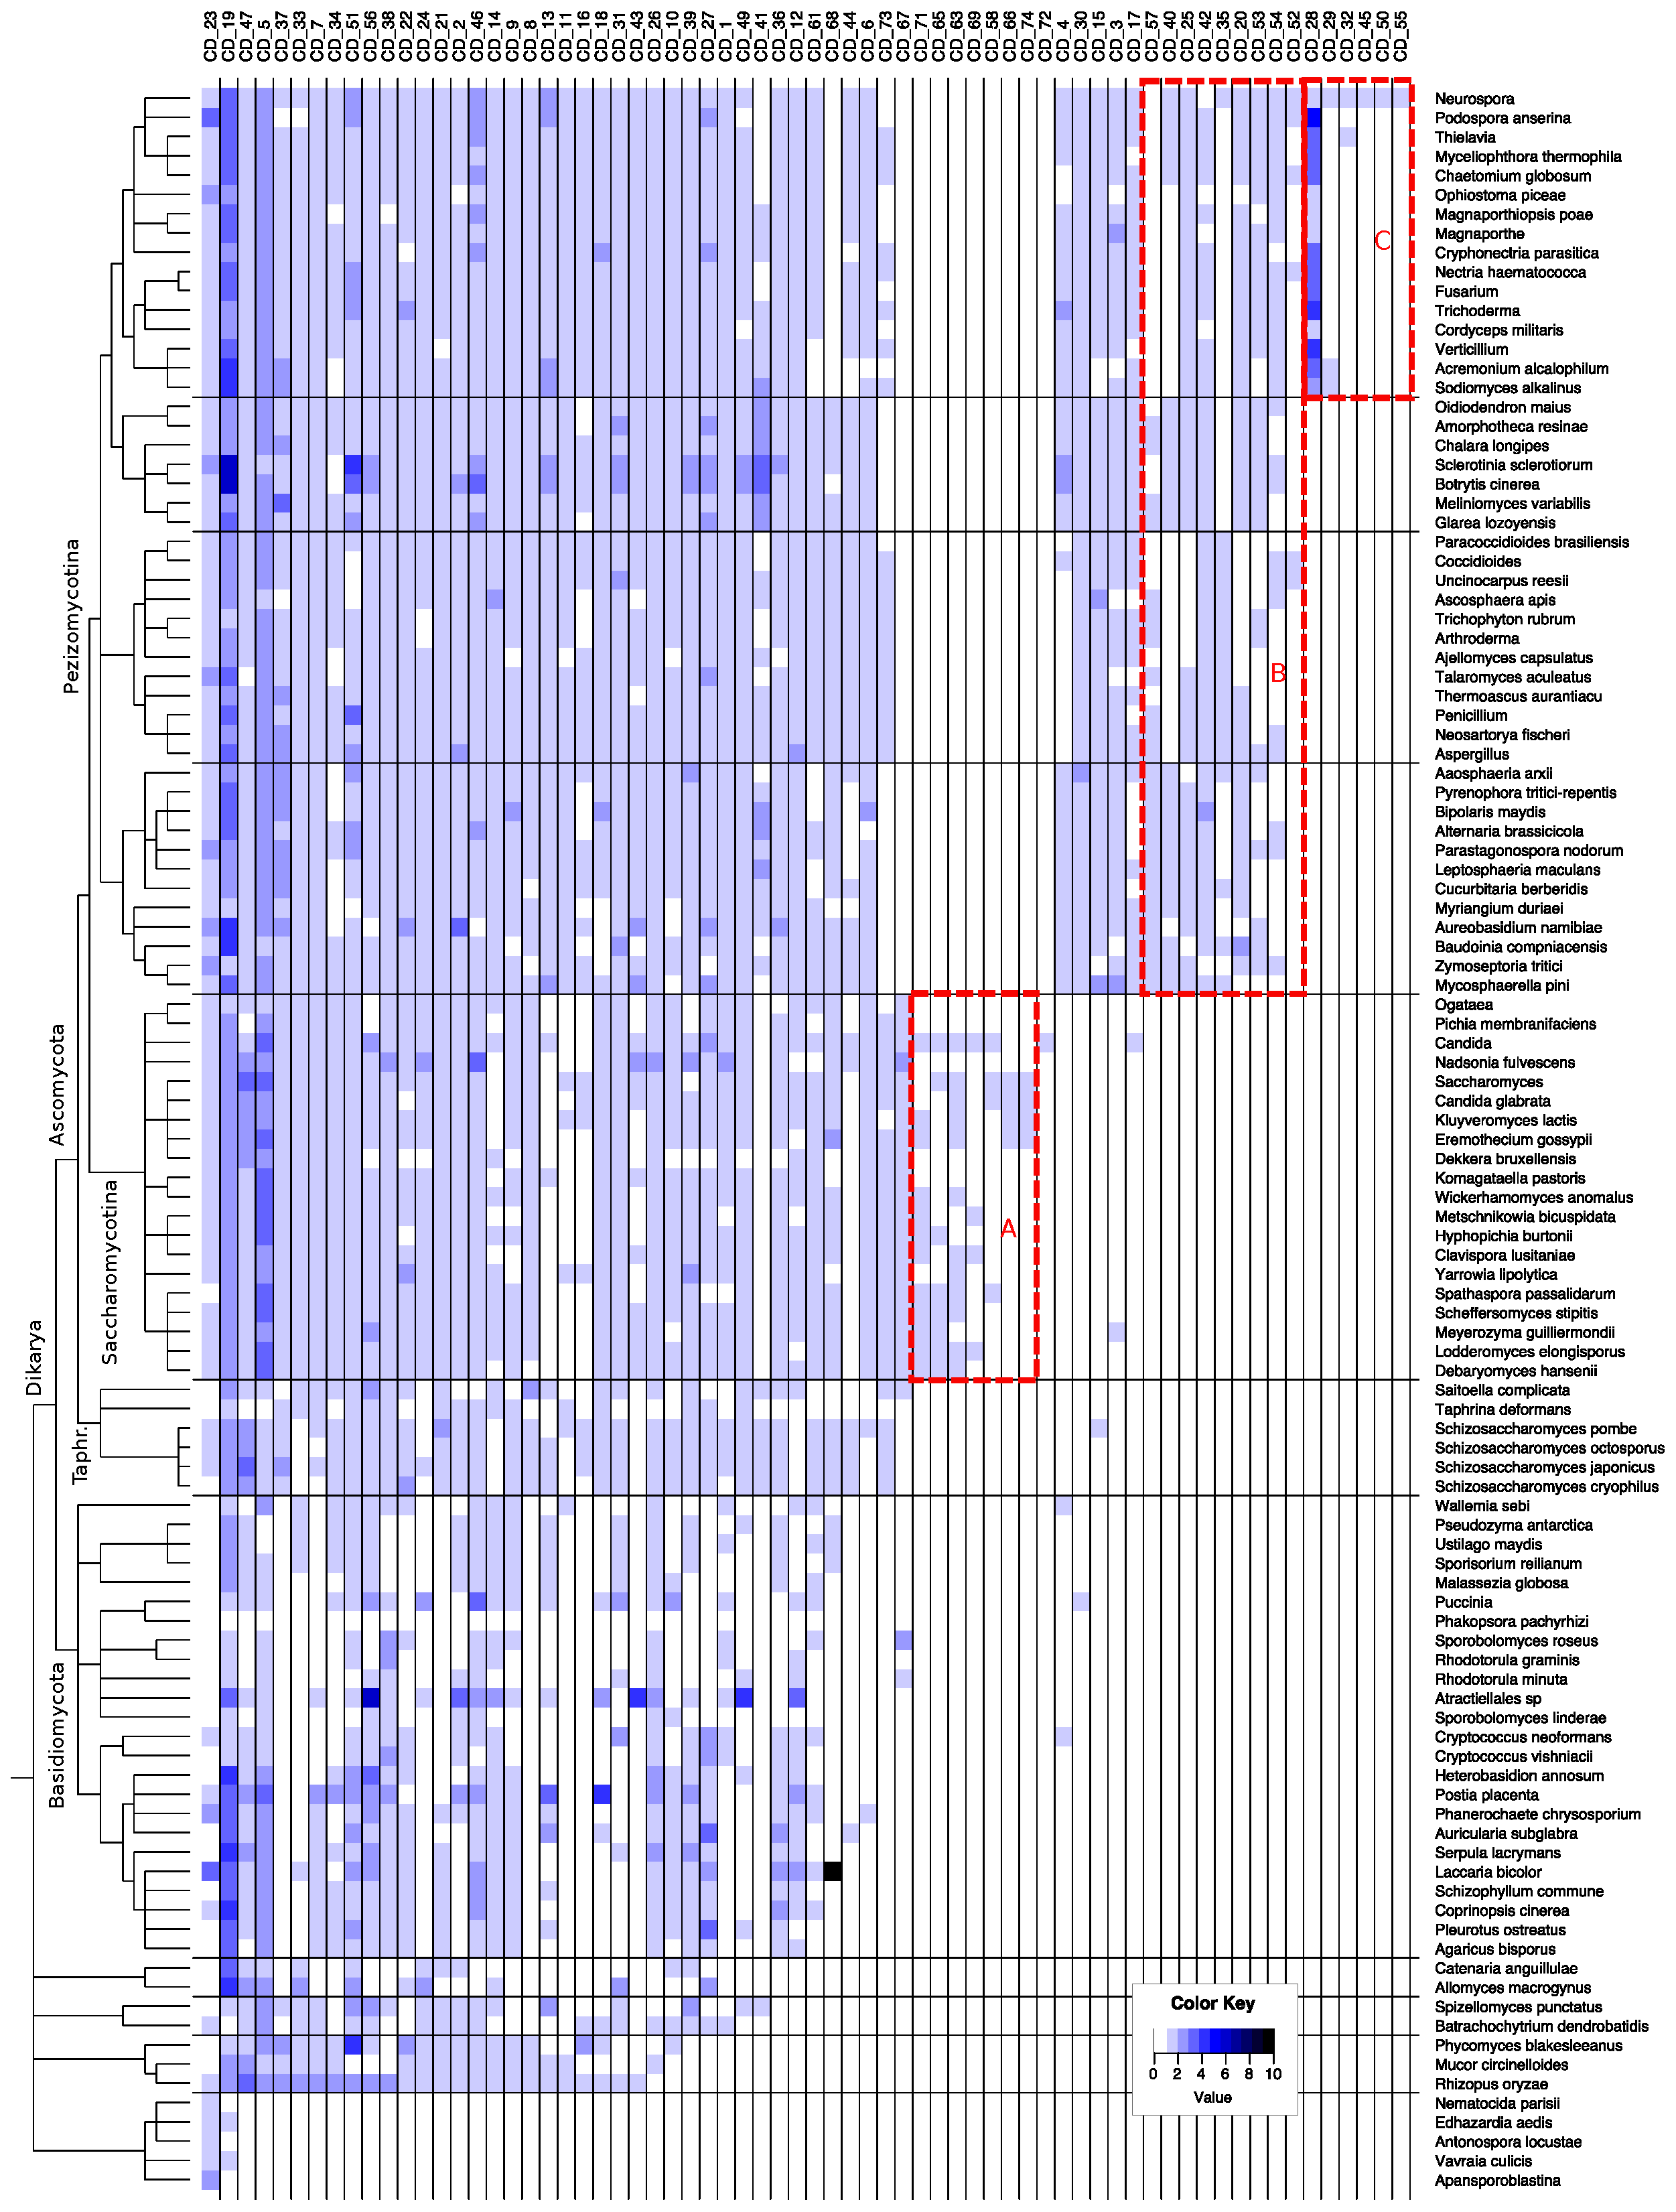
\includegraphics[width=1.05\textwidth]{pics/CD_snoRNAs_collapsed.eps}
  \caption{A heatmap of
    \snostrip-detected \cd s is shown on the previous site. Each column represents a specific \sno\
    family, while each row either represents a certain species or
    genus. A taxonomic classification is shown on the left hand side. The amount of
    \sno s detected in a specific species and \sno\ family is encoded in a
    blue color scheme. Lineage specific families are boxed (A:
    Saccharomycotina, B: Pezizomycotina, C: Sordariomycetes). %Single
%    \sno\ detections in lineages without any other predictions are either marked with 'X',
 %   '$\star$', or '!', depending on their family-specific functionality. For further details see text.
  }
  \label{fig:heatmap_CD_snoRNAs} 
\end{figure*}



Nearly half of all \cd\
families are traceable down to the root of fungi (32/68), i.e., at least one early
branching fungal lineage is attested to carry this \sno\
family, such as Microsporidia, Mucoromycotina, Chytridiomycota, or
Blastocladiomycota. Additionally, several families are found to be
lineage-specific, e.g., seven in Saccharomycotina (see box 'A' in
Figure \ref{fig:heatmap_CD_snoRNAs}), nine in Peiziomycotina (box
'B'), and six in Sordariomycetes (box 'C'). These lineages map exactly to the
clades where original \sno\ data originated from.

In contrast to lineage-specific families, lineage-specific losses of
\sno s is also detectable. Basidiomycota, for example, are not found
to contain orthologs of families CD\_8, CD\_16, or CD\_37, while in
Saccharomycotina, no trace is found of \sno s of family
CD\_41. Members of CD\_40 are not detected in Eurotiomycetes, while
Sordariomycetes are attested to miss homologs of families CD\_47 and
CD\_68. In some other cases, one or two representatives
are found in lineages where the remaining species do not contain this
particular family. In these lineages, only the analysis of target
interaction might answer the question whether this single \sno\ is
a true member of the family or merely an artifact.


%\mysubsection{Box H/ACA \sno\ Families}
%
%\begin{figure}
%  \centering
%  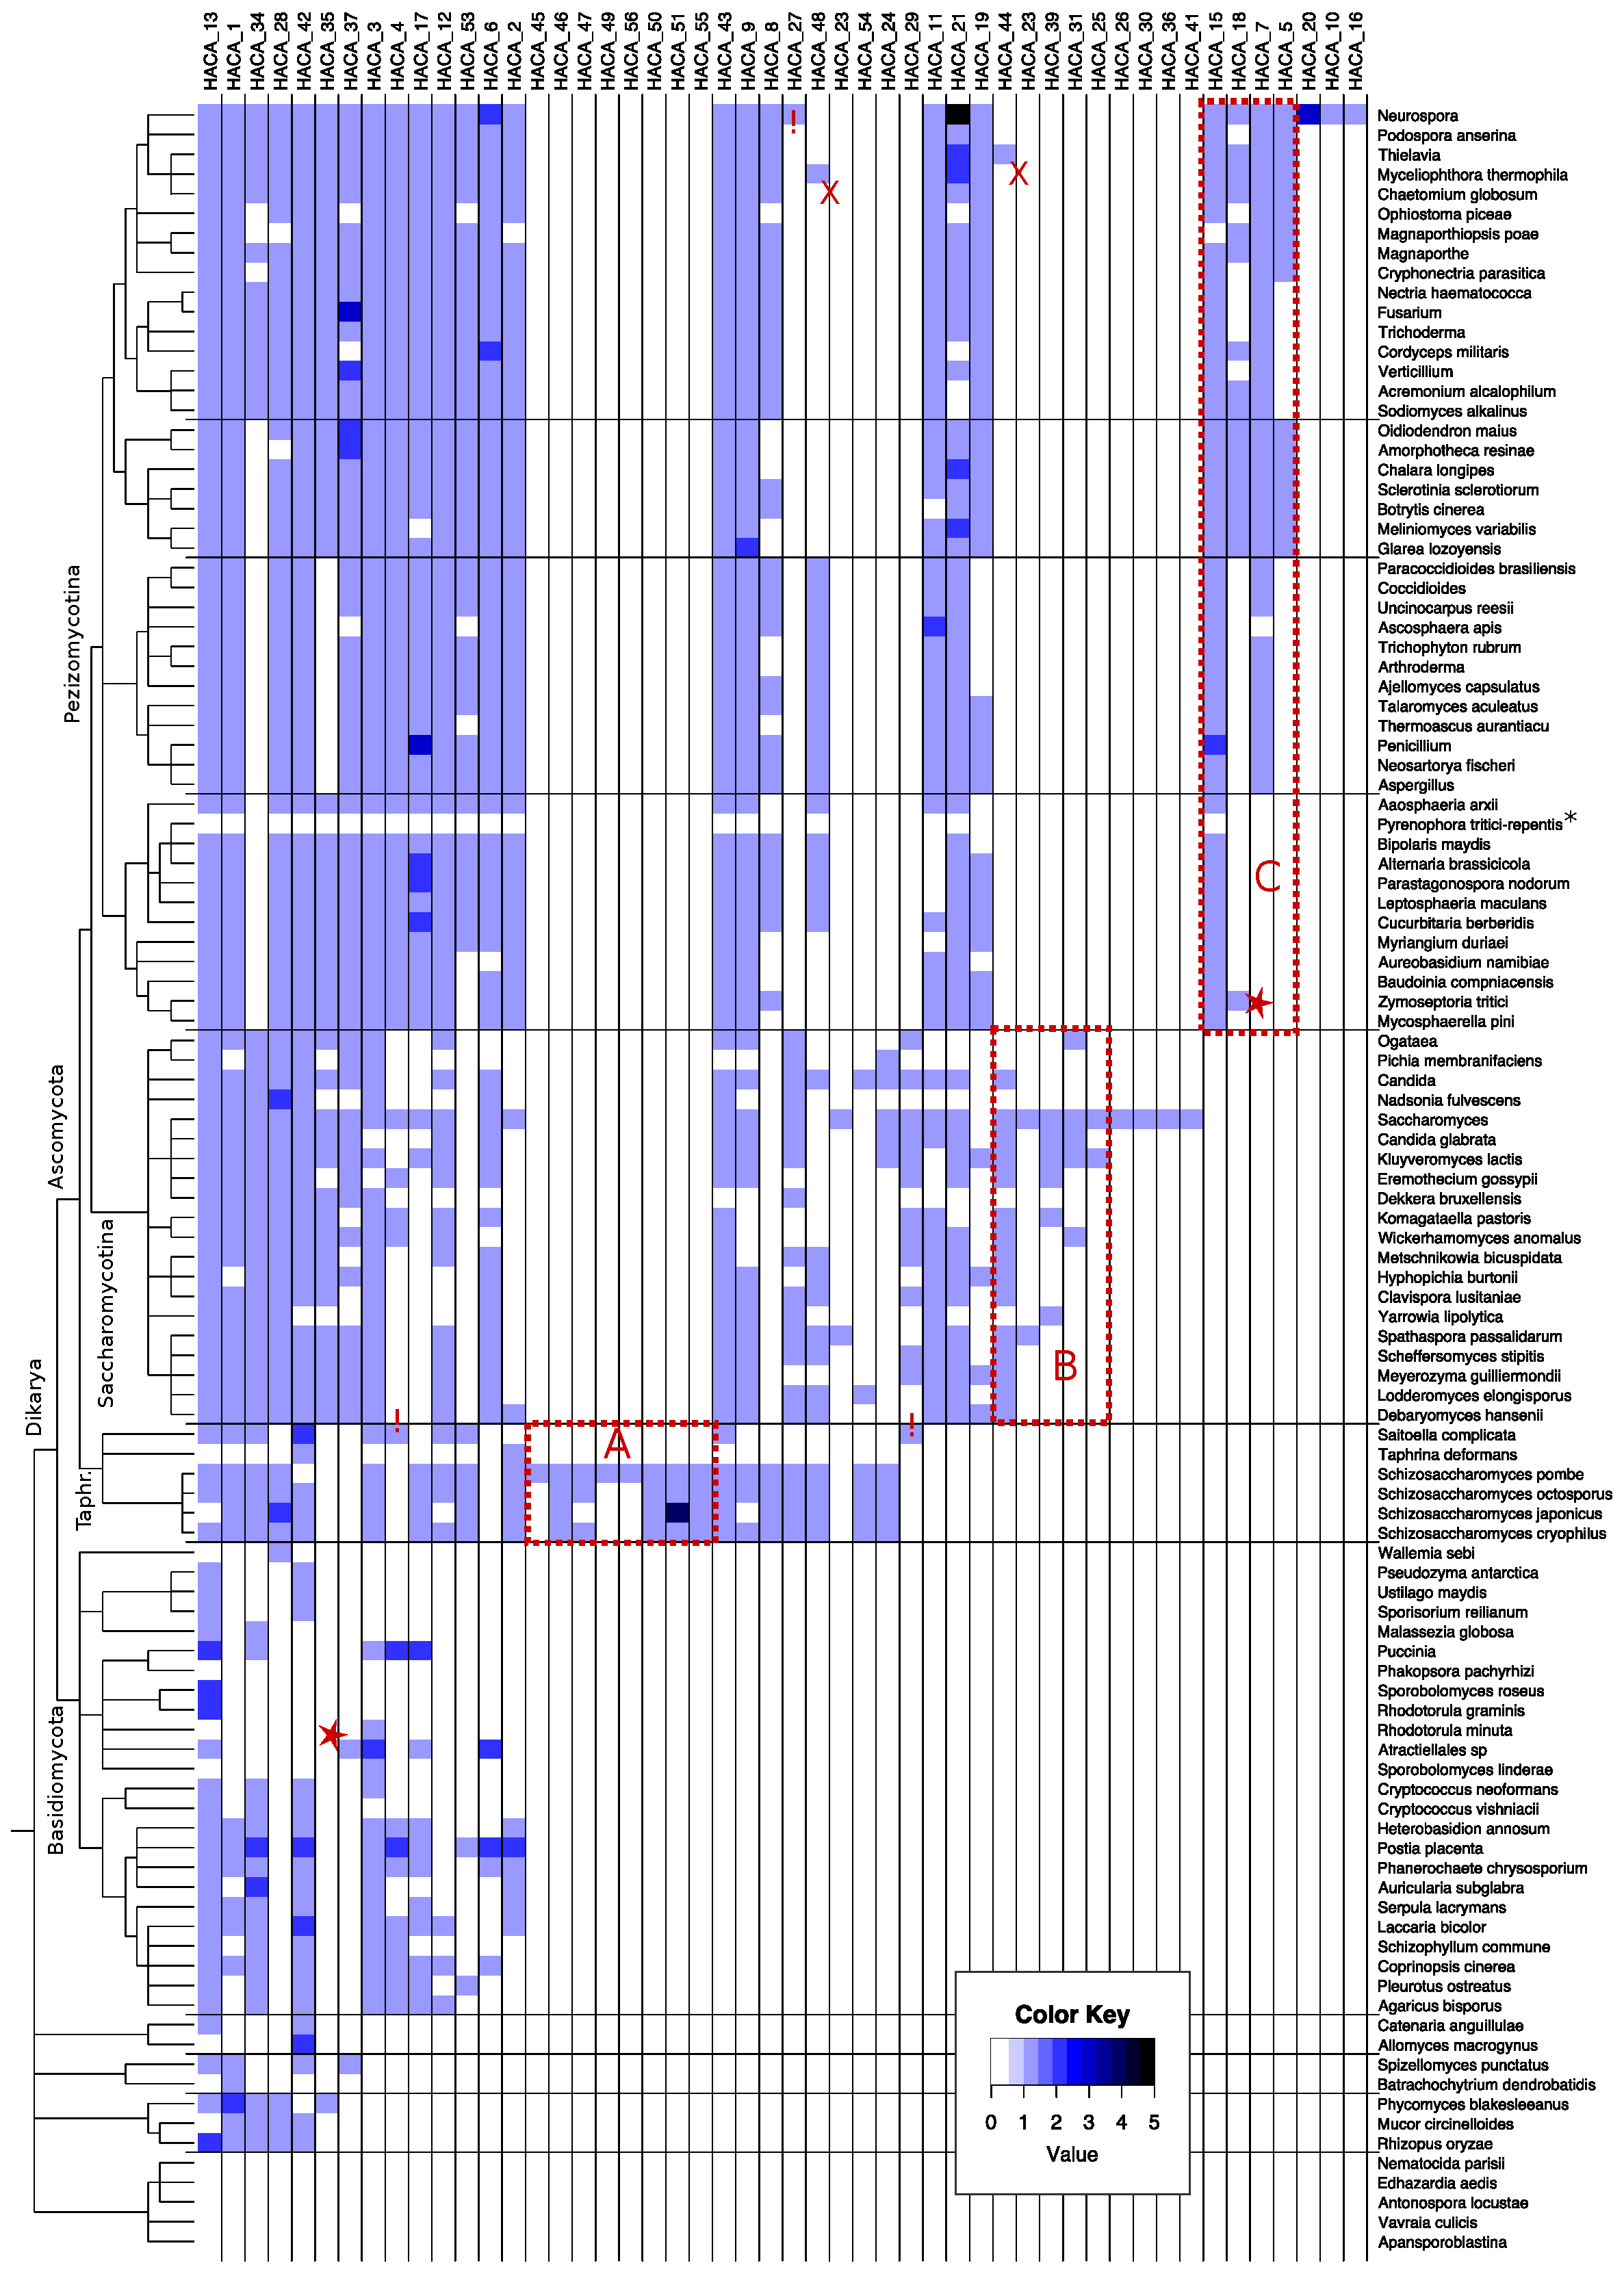
\includegraphics[width=\textwidth]{PICS/FUNGI/HACA_snoRNAs_collapsed.eps}
%    \caption{A heatmap of
%    \snostrip-detected \haca s is shown on the previous site. Each column represents a specific \sno\
%    family, while each row either represents a certain species or
%    genus. A taxonomic classification is shown on the left side. The amount of
%    \sno s detected in a specific species and \sno\ family is encoded in a
%    blue color scheme. Lineage specific families are boxed (A:
%    Schizosaccharomycotina, B: Saccharomycotina, C: Pezizomycotina). Single
%    \sno\ detections in lineages without any other predictions are either marked with 'X',
%    'star', or '!', depending on their family-specific functionality. For further details see text.}
%  \label{fig:heatmap_HACA_snoRNAs}  
%\end{figure*}

Compared to \cd s, only seven \haca\ families (out of 50) are detected in early branching fungi
and Dikarya. None of these is detected in Microsporidia
leaving this clade completely without any annotated \sno\ candidate. It
is apparent, however, that \haca s shows substantially
more lineage specific innovation and deletion events than observed in \cd s, see supplementary Figure.

%In total, seven families are exclusively found in Schizosaccharomyces
%(red box 'A' in Figure \ref{fig:heatmap_HACA_snoRNAs}),
%five in Saccharomycotina (red box 'B'), four in Saccharomyces, four in
%Pezizomycotina (red box 'C'), and two are exclusively present in Neurospora. 
In total, 22 out of 50 H/ACA families are merely found in a
small subset of species. Moreover, several families are found in two
or more lineages but seem to be completely lost in others, such as HACA\_33,
HACA\_56, and HACA\_24. They are present in Taphrinomycotina and
Saccharomycotina but cannot be found in Pezizomycotina. 
%In other families it
%occurs that just a single \sno\ molecule is detected amongst all organisms
%of a particular lineage raising the question whether this sequence is
%indeed functional or the remains of the vanished \sno\ gene. Several
%such cases are marked in Figure \ref{fig:heatmap_HACA_snoRNAs}. Furthermore, their target binding ability is classified to better capture the
%implication made by these single \sno: Categories are 'non-functional'
%(red 'X'), i.e., the \sno\ is not predicted to bind the conserved and annotated
%target, 'marginal functional' (red '$\star$'), meaning that the predicted
%mfe is above -30 kcal/mol, or 'highly  functional' (red '!') stating
%that the family specific target region can be bound extraordinary
%well. In seven detected cases, two are found to be non-functional, two
%are found to be functional with a minimum free interaction energy
%above -30 kcal/mol, while the remaining three sequences are predicted to bind
%the target region exceptionally.


\begin{figure*}
  \centering
  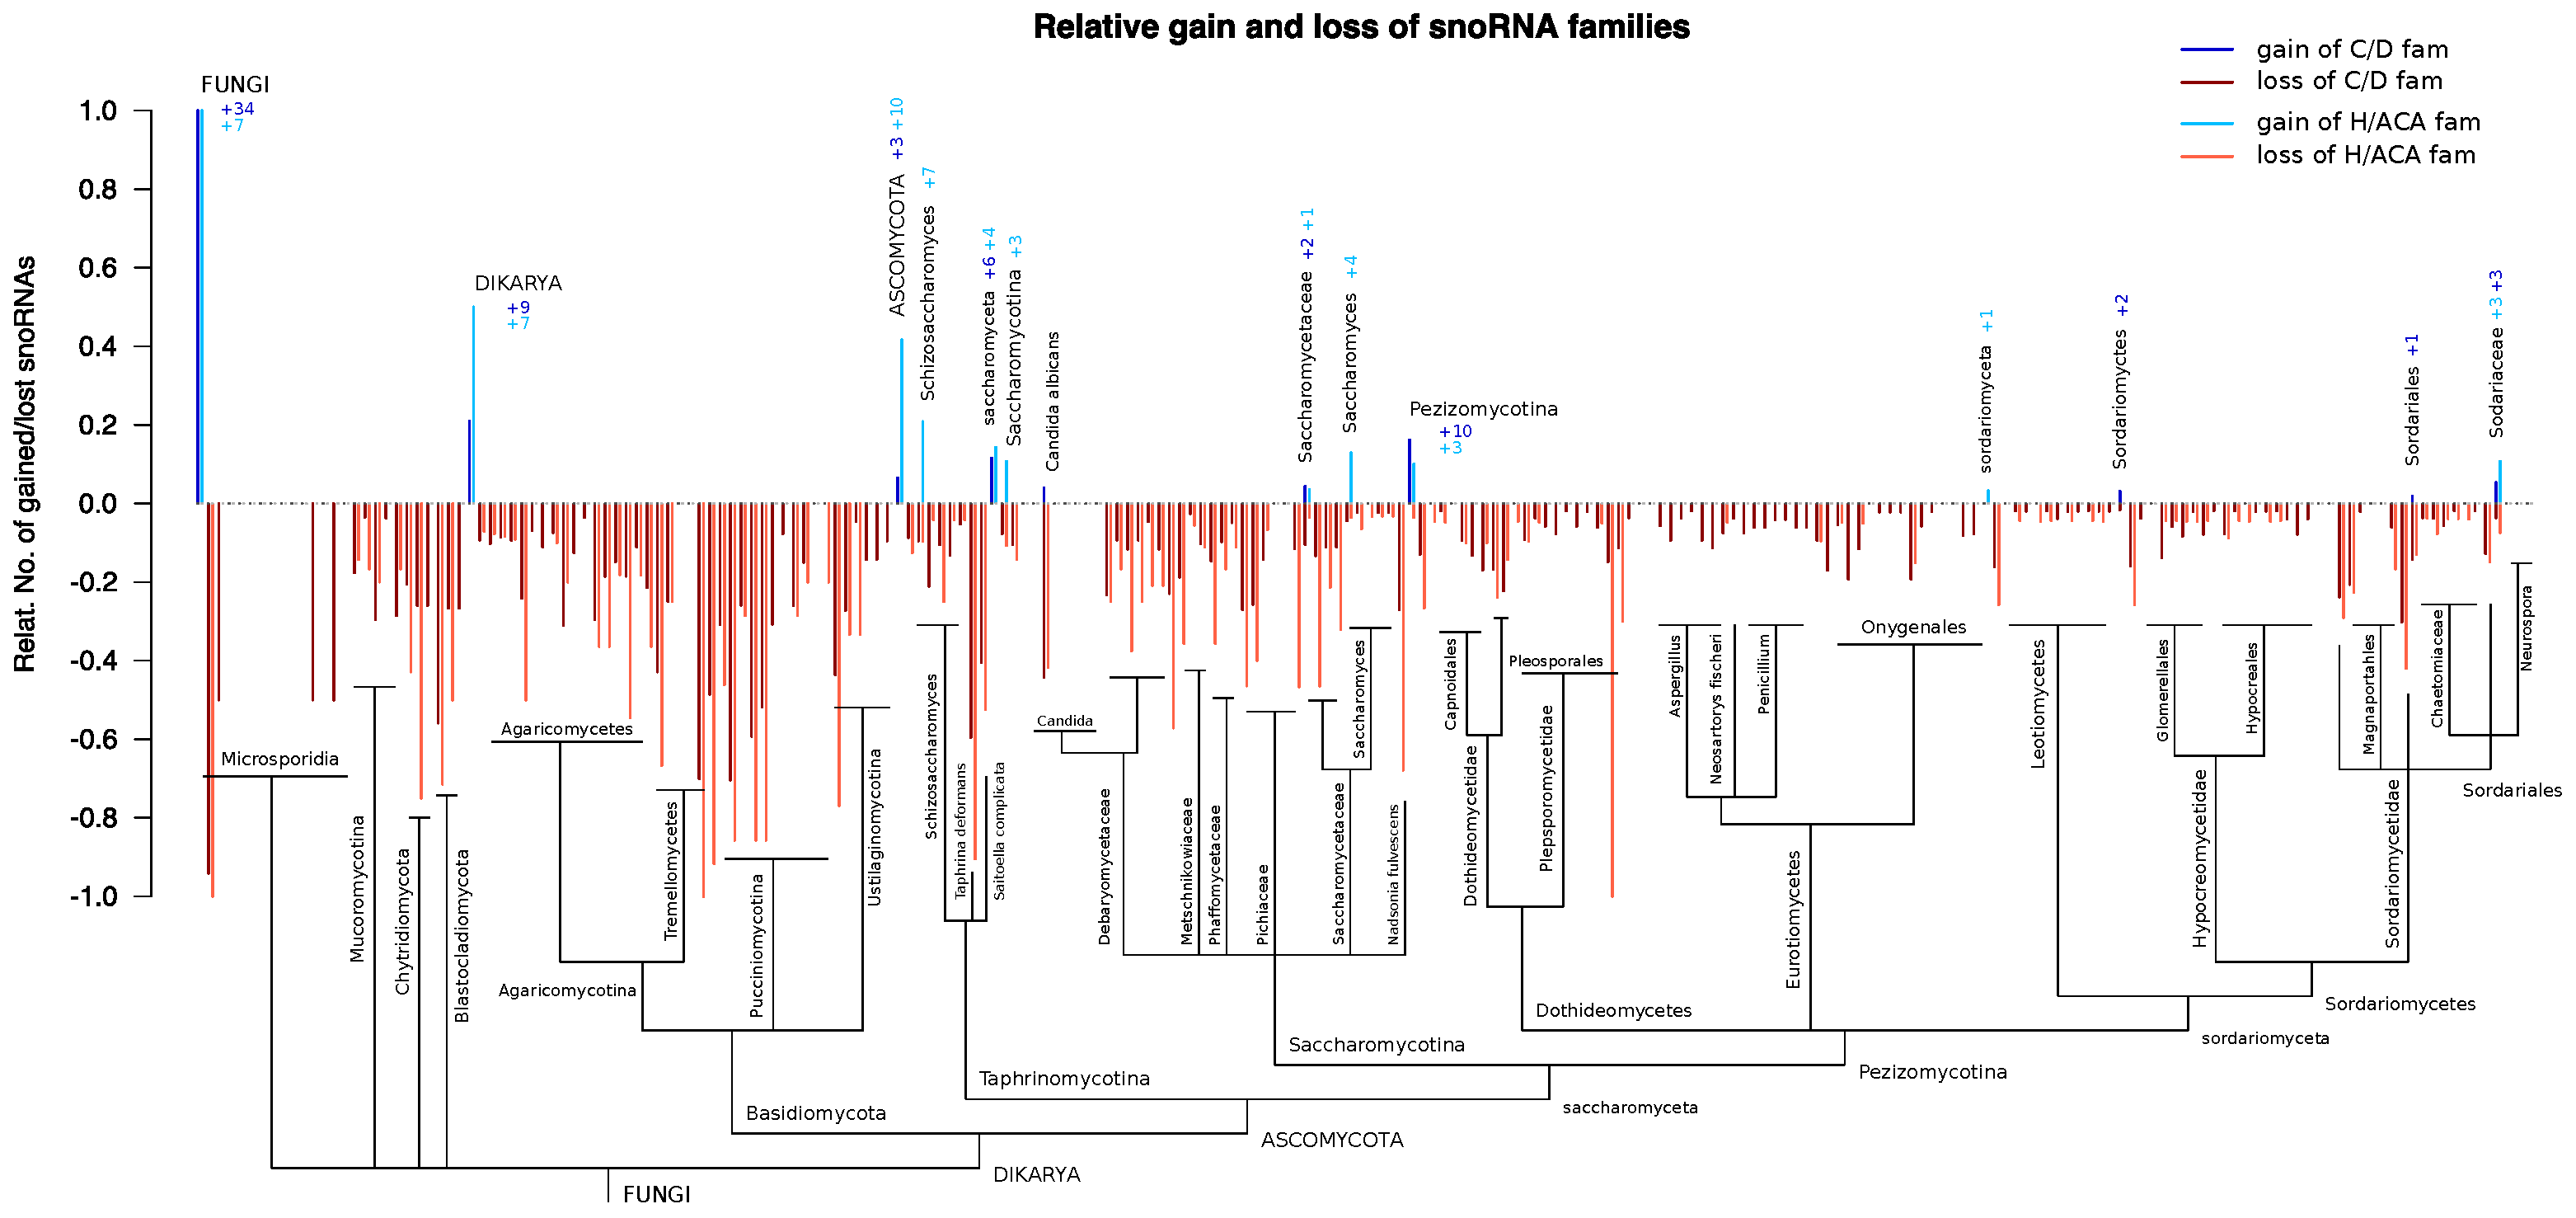
\includegraphics[width=\textwidth]{pics/fungi_relative_gain_loss.eps}
  \caption{Relative number of gains and losses of entire snoRNA families during fungal
evolution. The relative gain is the number of gained snoRNA families compared to the
observed number of snoRNA families. The relative loss describes the number of lost
snoRNA families compared to the number of snoRNA families in the parent node of the
phylogenetic tree.}
\label{fig:relative_innovation_deletion_events}
\end{figure*}


Another noticeable observation is that not a single \haca\ is
found in \Ptt\ (marked with an asterisk in the supplement Figure). This stands in sharp contrast to C/D \sno\ sequence,
where \ptt\ orthologs are found in nearly all families that are
present in the \ptt-containing Dothideomycetes lineage.


\paragraph{\textbf{Evolutionary events in snoRNA history}}

Relative innovation and deletion events mapped to the pre-ordered
nodes of the NCBI-derived taxonomic tree up to species level are shown in
Figure \ref{fig:relative_innovation_deletion_events}. 
Absolute events that are traceable from the root of major fungal
lineages up to families and orders are shown in the supplement.
In both images, it is clearly
visible that a large amount of \sno\ families has evolved at each
major branch point along the backbone of the taxonomic
tree. In case of \cd s, 34 families are already present at the root of
fungi, indicating an even more ancient origin. At the root of 
Dikarya, Ascomycota, Saccharomyceta, and Pezizomycotina, a total
 of 9, 3, 6, and 10 families arose, respectively. A similar picture is drawn in
case of \haca s where 7 families are already present at the root of
fungi and additional 7, 10, 4, and 3 families are gained at the root
of Dikarya, Ascomycota, saccharomyceta, and Pezizomycotina,
respectively. Due to the homology-based search procedure in \snostrip\
which is based on a experimentally verified set of \sno s, it is quite
logical that innovation events are exclusively detectable at nodes
leading to the leaves that represent these five species.  



Major \sno\ losses in both, an absolute and relative point of view,
can be seen in Microsporidia which are found to harbour only two
distinct \cd\ families while all remaining C/D and H/ACA families are
not detectable. Gardner \emph{et.~al} formerly mentioned the
remarkable absence of \sno\ genes in this clade, although all
components of the \sno\ machinery are clearly present
\cite{Gardner:2010}. They argued with a lack of experimental
investigations and only insufficient bioinformatic methods. However,
the more sophisticated \snostrip\ approach was also not able to detect
a great variety of \sno\ genes which might point at a rather
diversified \sno\ repertoire compared to other fungal lineages. 
%On the
%contrary, losses of seven or more families at a particular point in
%the tree, have only a little relative effect when a large fraction of
%\sno\ families has been gained before, cf. losses of Dothideomycetes
%(-8 C/D, -8 H/ACA) and Eurotiomycetes (-7 C/D, -10 H/ACA) in the
%Figure \ref{fig:relative_innovation_deletion_events}. 

When focusing on species level, it is frequently observed that single
organisms seem to have lost a large amount of their snoRNA repertoire. In
particular, species in the Basidiomycota lineage miss a fairly high
portion of their \sno s. Especially \wse\ and several Pucciniomycota
seem to have lost nearly their entire set of \haca s (\wse: 0.92, \rmi: 0.86,
or \sli: 0,86). The impact on \cd s is more moderate (0.26 on
average). A potential correlation with significantly smaller genome
sizes in Pucciniomycota was not detected (data not shown). The
previously mentioned loss of the entire \haca\ set in \Ptt\ is also clearly
visible. Other organisms such
as \pan\ and  \opi\ also show an increased loss rate (\pan: 0.15 C/D
and 0.13 H/ACA; \opi: 0.30 C/D and 0.42 H/ACA). 

%\begin{figure}
%  \centering
%  \includegraphics[width=0.95\textwidth]{PICS/FUNGI/taxonomic_tree_ncbi_collapsed.eps}
%  \caption[Innovation and Deletion events in fungal \sno\
%  history.]{Innovation and deletion events in fungal \sno\ evolution.}
%\label{fig:absolute_innovation_deletion_events}
%\end{figure}

\paragraph{\textbf{Novel \emph{Candida albicans} \sno s are lineage-specific}}

%To investigate the fate of intron encoded ncRNAs in species that
%suffered massive intron loss, Mitrovich \emph{et.~al} identified novel \sno\ sequences in different
%species including \calb\ based on \emph{de novo} prediction and
%expression values \cite{Mitrovich:2010}. For \calb, 40 potential \cd\
%sequences were annotated and 36 of them showed high sequence similarity
%to known budding yeast \snos. One of the remaining sequences shares a homologous target
%binding region with a known \ncr\ \sno\ (CD\_39), while the other three
%candidates combine no obvious homology to already published \snos. 
%
%Family CD\_69 (LSU-C2809 in \cite{Mitrovich:2010}) is found in all other \emph{Candida} organisms and two additional
%Saccharomycotina. The initially predicted
%target interaction with 25S-4055 (\calb: 25S-3118) is also highly
%conserved across all identified \snos\ (ICI score: 1.813).
%Homologs of the \calb\ sequence CD\_71 (LSU-G1431) were successfully
%traced in most Saccharomycotina, except for Saccharomycetaceae. The
%extraordinary ICI score of 1.289 indicates a highly conserved target
%binding capability with position 25S-2490 (\calb: 25S-1740).
%The third novel \sno\ candidate CD\_72 (LSU-G364) was merely detectable in two closely related
%species, \cdu\ and \ctr, respectively. Although all three sequences
%show a highly conserved target region upstream of box D, it is not
%possible to reliably identify a conserved target interaction based on
%such a small set of closely related organisms. 
%%This is due to conserved \snos\
%%on the one hand and, obviously, highly conserved target RNAs on the
%%other hand. This makes each predicted interaction that is traceable in
%%a single organisms
%% also traceable in the other species. In case of this particular
%% family, 
%Six potential target
%interactions have an ICI score above 0.9 although their mean minimum
%free binding energy is relatively high (between -7.3 and -9.0).
%
%%Please note that the originally denoted modification sites are
%%not equal to the \calb\ specific modification sites published here since
%%different 25S rRNA sequences have been used. The authors named their
%%novel identified sequences with respect to their target predictions
%%but die not provide the corresponding targetRNA sequences. 
%


Mitrovich \emph{et.~al} identified four novel \sno\ candidates among their set fo 40 \sno\ genes that showed no high sequence similiarity towards already annotated budding yeast sequences \cite{Mitrovich:2010}. One of these sequences is found to share a homologous target
binding region with a known \ncr\ \sno\ (CD\_39). Families CD\_69 (LSU-C2809 in \cite{Mitrovich:2010}) and CD\_71 (LSU-G1431)  are exclusively present in Saccharomycotina except for Saccharomycetaceae. They are also found to share an extraordinary conserved target-interaction with ICI scores of 1.813 (25S-4055; \calb:~25S-3118) and 1.289 (25S-2490; \calb:~25S-1740), respectively. The remaining family CD\_72 (LSU-G364) is merely found in two closely related species: \cdu\ and \ctr.



\paragraph{\textbf{Fission Yeast Specific \sno s}}

%Similar to \calb, several \sno s published in the fission
%yeast \cite{Li:2005} are found to be lineage or even species
%specific. HACA\_46 (AJ632008 in \cite{Li:2005}) is annotated to be a double guiding \sno\ and shows
%indeed two conserved pseudouridylation pockets in both hairpins across
%the four members of Schizosaccharomyces. The predicted modification
%site for hairpin 1 (HP1) is also known to be modified in \sce\ (25S-2314) and
%human. The correspondung budding yeast family HACA\_36 (snR86),  
%which is experimentally confirmed to guide
%pseudouridylation at this precise position, is merely a functional
%homolog to the Schizosaccharomyces specific HACA\_46 \sno\ since
%the functional target binding site resides in hairpin 2 (HP2) instead of the first
%hairpin. A similar situation is found in HACA\_47 that shares a
%conserved and annotated HP2 target (25S-2060). This position is again
%known to be modified in both budding yeast and human. But although both
%anti sense elements (ASE) are located in hairpin two in \spo\ and \sce\, sequences of both
%groups share far too little sequence similarity to be denoted as homologous
%families on sequence level. However, they are clearly functional homologs. 
%
%While families HACA\_50 and HACA\_55 are present in all
%Schizosaccharomyces species the true modification site remains
%secret. The putative target in  \sno\ HACA\_50 was neither
%found to be conserved in other Schizosaccharomyces and
%conserved predictions for the orphan target sites in HACA\_55 have not
%been detected by \snostrip.  
%
%The three sequences HACA\_45, HACA\_49, and HACA\_56 are exclusively
%found in \spo. The correct assignment of a functional modification
%site is nearly impossible for single sequences, and hence these
%originally orphan guides remain orphan.
%
Similar to \calb, several \sno s published in the fission
yeast \cite{Li:2005} are found to be lineage or even species
specific. In the original publication, 12 sequences have not been mapped to budding yeast \sno s and 7 of them have no predicted target interaction. By means of \snostrip, HACA\_46 (AJ632008 in \cite{Li:2005}) and HACA\_47 (AJ632011) have been detected to be functional homologs to HACA\_36 (snR86) and HACA\_27 (snR5), respectively. The first one includes a switch from a HP1 target in \spo\ to a HP2 target in \sce, while the latter two families share far too little sequence similarity to be denoted as homologous sequences. Families HACA\_9 (AJ632018), HACA\_48 (AJ632010), HACA\_53 (AJ632016), and HACA\_54 (AJ632012) are found to be conserved outside of Taphrinomycotina. The first two families map to families with an annotated target while the latter families lack such a finding. The remaining sequences are either specifically detected in Schizosaccharomyces (HACA\_50 (AJ632009), HACA\_51 (AJ632017) and HACA\_55 (AJ632013)) or exclusively found in \spo\ (HACA\_45 (AJ632015), HACA\_49 (AJ632019), and HACA\_56 (AJ632014)).


%\TODO{
%What happened to  AJ632018?? mapped to HACA\_52, but lost somehow...
%Mapped to HACA\_9, but mapping was lost...
%\Spo\ sequences that were not mapped originally to already annotated budding yeast sequences: AJ632008 - AJ632019. AJ632008-AJ632012 have predicted, annotated target interactions. the remaining families are denoted as orphan.
%
%HACA\_46 (AJ632008) and HACA\_47 (AJ632011) are functional homologs to budding yeast annotated sequences. 
%
%
%HACA\_50 (AJ632009), HACA\_51 (AJ632017) and HACA\_55 (AJ632013) are found in all Schizosaccharomyces, but lack confident prediction of target interaction. 
%Sequences HACA\_45 (AJ632015), HACA\_49 (AJ632019), and HACA\_56 (AJ632014) are exclusively found in \spo. 
%
%Conserved outside of Taphrinomycotina with an annotated target: HACA\_48 (AJ632010), HACA\_9 (AJ632018).
%conserved outside of Taphrinomycotina with unannotated target prediction: HACA\_53 (AJ632016), HACA\_54 (AJ632012)
%
%What about the remaining 5 snoRNA candidates - HACA\_48 (AJ632010), HACA\_51 (AJ632017), HACA\_9 (AJ632018), HACA\_53 (AJ632016), and HACA\_54 (AJ632012)?
%
%% HACA\_48 conserved in Taprhino, Saccharom, Dothideom, Eurotiom. ICI: 1.15 annotated
%% HACA\_51 conserved in Taphrino, 18S-400 in two of four organisms, ICI: 0.48 HP2
%% HACA\_9 conserved in Ascomytcota, HP1 target: 25S-1962, ICI 1.17 HP1, annotated target
%% HACA\_53 conserved in Taphrino, Pezizomycotina, potential target 18S-1302, ICI 0.82, not annotated
%% HACA\_54 conserved in Taphrino, candida, debaryomyces, potential targte found: 25S-3439, ICI 1.22
%
%
%
%}



\subsection{Conservation of Target Interaction}

In accordance to their conserved function, each
\sno\ family can either be classified as single guide, double guide,
or orphan \sno. Single guide sequences share a conserved and
functional anti sense element either upstream of box D or D' in \cd\
or either in hairpin 1 (HP1) or hairpin 2 (HP2) in \haca s. Double
guide \sno s exhibit functional target binding
regions in both positions. Orphan \sno s have no known and conserved
target interaction. Normally, each individual \sno\ is predicted to be capable of binding
several regions of different targetRNAs. But target predictions that
are based on single sequence predictions
are not overly convincing in a biological point of view. 

\begin{figure*}
  \centering
  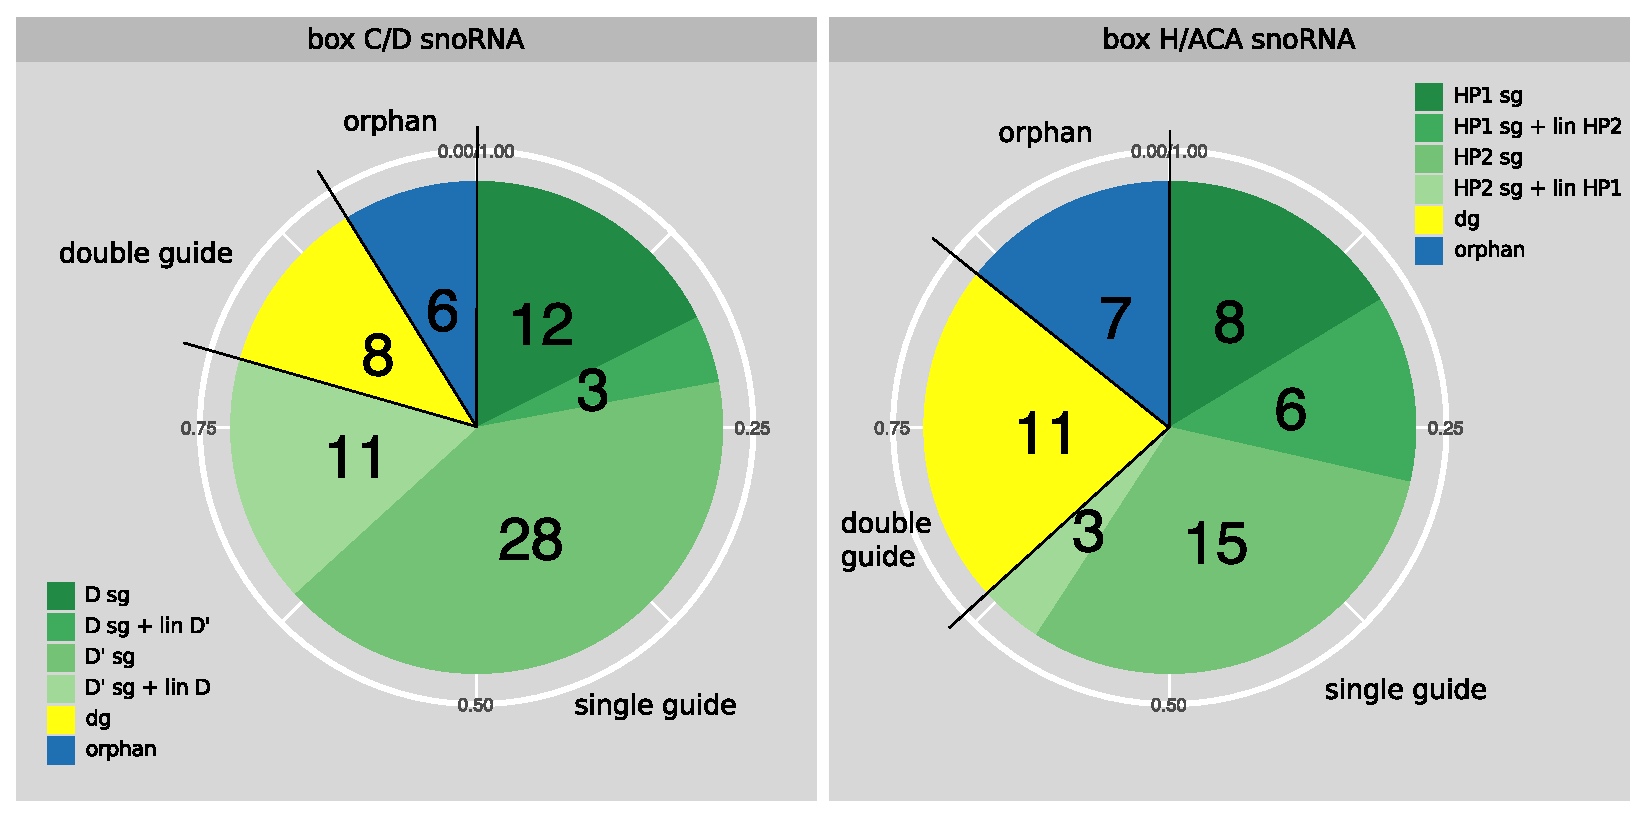
\includegraphics[width=0.9\textwidth]{pics/pieCharts_snoRNAs_modified.eps}
  \caption[Classification of \sno\ families as single or double guides.]{Pie
    chart of both major \sno\ classes. A \sno\ family is classified based on
    its conserved target prediction either as single guide (sg), single
    guide with a lineage specific target in its non-conserved target
    region (lin),
    double guide (dg), or orphan.}
  \label{fig:pie_charts}
\end{figure*}

Within the 68 \cd\ families, the large majority (40) is found to be
\textit{true} single guides. 28 families share a functional D' target
and the remaining 12 families a conserved D box associated binding
site. An additional amount of 14 \cd\ families are \textit{predominantly}
found to be single guides, i.e., these families share exactly one highly
conserved target binding region (three families share a conserved D target
while 11 families share a functional D' target), whereas the other
target region is only found to be functional in subset of
organisms. Eight families harbor two
functional target binding regions that are conserved throughout all
lineages where these families are detected. 
Six families
 are originally denoted as orphan \sno\ meaning that no potential interaction has been
 published thus far. In case of \haca s, 23 families are \textit{true}
 single guides: 8 families share a conserved pseudouridylation pocket
 in hairpin 1 and 15 families share a HP2 target. Further 6 families
 comprise a lineage specific HP2 target besides their overly
 conserved target in hairpin1. The opposite situation can be seen in 3
 \haca\ families. 11 families are found to be double guides, while 7
 families are orphan. A summary of the \sno\ classification can be seen
 in Figure \ref{fig:pie_charts}.  Detailed information about each family and the
 \snostrip-assigned target interactions, e.g., alignment position of
 the modification site, ICI scores, and mean minimum free energy
 values, can be found in the supplement. 


%%%%%
%% DOUBLE GUIDE SNORNAS
%%%%%
Solely a minority of \cd s is found to contain two overly
conserved target regions upstream of box D and D'. However, except for
CD\_5 and CD\_19, none of
the remaining six families is traceable amongst all major fungal
lineages. Two families, CD\_17 and CD\_35, are found in Pezizomycotina
while CD\_67 is exclusively found in Saccharomycotina. The remaining
families are either found in Sordariales (CD\_32), a subgroup of
Sordariomycetes, or in Glomerellales and Neurospora (CD\_29). 

Double guide \haca\ families occur more frequent. 11 families are originally annotated as
double guides and most of their targets are convincingly confirmed
by \snostrip. Furthermore, double guided \haca s are commonly traceable across a wide
range of fungal organism. Four families have their origin at the root of Dikarya or
even further back (HACA\_2, HACA\_3, HACA\_6, HACA\_37). Two more families are traced to the root of
Ascomycota (HACA\_27, HACA\_29), whereas the remaining five families are lineage (two
found in Saccharomycotina, HACA\_31, HACA\_39) or genus specific (two found in
Saccharomyces, HACA\_26, HACA\_30; one found in Schizosaccharomyces, HACA\_46).

Family HACA\_3 is published to guide three targets in both the budding yeast
and fission yeast (annotated as snR3 in \sce, AJ632000 in \spo);HP1 is known to guide modification at position 25S-3311 (25S-2129 and
25S-2216 in the budding and fission yeast, respectively), while there
are two targets in HP2; 25S-3449 and 25S-3315 (\sce\ 25S-2264 and
25S-2133, \spo\ 25S-2351 and 25S-2220). All three targets are found to
be conserved across Dikarya. In the original Neurospora publication,
however, HP1 is annotated to guide the isomerization at position
25S-1200 (25S-401 in \Ncr). This guiding capability is not found to be
conserved throughout the members of this family unlike the yeast
annotated target which is also convincingly predicted in Neurospora
species, even with a lower interaction energy. 

\paragraph{\textbf{Orphan \sno}}
Orphan \sno s are sequences without a known target interaction on both
potential anti sense elements. In the originally published \sno\ datasets of five different fungi, orphan \cd s were annotated for \sce\
(2), \ncr\ (2 sequences), and \afu\ (9). In addition to these sequences,
11 \ncr\ \sno s have been published with predicted targets
based on single sequence target prediction only. Since there is
usually more than just one valuable prediction for a single \sno, these predictions might be
misleading until they are evaluated under the light of
evolutionary conservation or the original \sno\ sequences are mapped to species with verified
targets.

A detailed summary of these sequences and their predicted targets with
respect to evolutionary conservation is shown in the supplement. Highly conserved
target interaction that are predicted by \snostrip\ are shown in Table \ref{tab:orphan_cd_snoRNAs_short}. 

\begin{table}
  \caption{Assigning putative targets to previously
    orphan \cd s. Families that do not contain sequences with
    experimentally verified targets are marked with '*'. }
  \label{tab:orphan_cd_snoRNAs_short}
  \begin{center}
    \begin{footnotesize}
      \begin{tabular}{c|c|c|c|c}
      original&&target&&snostrip\\
      name&\raisebox{1.5ex}[-1.5ex]{box}&position&\raisebox{1.5ex}[-1.5ex]{ICI
      score}&name\\
  \hline
  Nc CD\_10&D'&18S-479&1.13&CD\_10\\
\hline
  Nc CD\_26&D'&25S-3836&0.86&CD\_26\\
\hline
  Nc CD\_53&D'&25S-3500&0.71&CD\_53*\\
\hline
  Nc CD\_54&D'&U60-70&1.43&CD\_54*\\
 \hline
  AM921936&D'&25S-4198&1.50&CD\_36\\
\hline
  AM921937&D'&18S-479&1.13&CD\_31\\
\hline
  AM921938&D'&25S-3474&1.19&CD\_7\\
\hline
  AM921939&D'&18S-179&1.09&CD\_15*\\
\hline
  AM921940&D&18S-849&1.21&CD\_41*\\
\hline
  AM921941&D'&18S-630&1.36&CD\_24\\
\hline
  AM921942&D&18S-456&1.71&CD\_37\\
\hline
  AM921944&D'&18S-1083&1.57&CD\_49\\
\hline
  AM921945&D'&25S-3836&0.86&CD\_26\\

    \end{tabular}
    \end{footnotesize}
  \end{center} 
\end{table}

Unfortunately, potential targets for both orphan \ncr\ \sno s are not
unambiguously discovered by \snostrip. The best prediction yields an
ICI$_{sno}$ score of 0.71 for family CD\_53 and is loosely found in
several Pezizomycotina species (25S-3500, mean mfe: -11.56). The
second family (CD\_55) is exclusively found in Neurospora preventing a
functional analysis of potential targets based on conservation aspects. 

In case of both budding yeast \sno s (snR4, snR45), no potential target is found
across canonical target sequences, although family snR4 is found to be
present in several fungal lineages such as Taphrinomycotina,
Saccharomycotina, and several Pezizomycotina species. Family snR45, on
the other side, is exclusively found in Saccharomycetaceae.

The picture looks much better in case of \afu\ orphan \sno s. The
\snostrip\ pipeline was able to map seven out of nine orphan \cd s
to families with experimentally validated targets. These target
interactions are also predicted in \afu. Both remaining families
(marked with '*' in Table \ref{tab:orphan_cd_snoRNAs_short}) are
traceable in the majority of Pezizomycotina species and putative
target sites are also conserved making the \snostrip\ results
plausible despite a missing experimental verification.

The set of 11 \ncr\ \sno s, with predicted targets but without homologous
relations to other known \sno s,
comprised 16 distinct targets published in the original publication \cite{Li:2005}.
Ten of these targets were confirmed by conservation using \snostrip.
Three targets were annotated as tRNA modification
sites and hence, are not checked in this study. However, these target
regions show no conserved and obvious base pairing capabilities to
canonical target RNAs such as rRNAs or snRNAs. The remaining three
target sites were predicted based on falsely detected D' box
motifs and thus, are neither biologically correct nor conserved across
species. In two cases, evolutionary conserved box motifs are
identified and convincing target sites are predicted by \snostrip\
(CD\_10, D' target, ICI: 1.13; CD\_26, D' target, ICI: 0.86), see Table
\ref{tab:orphan_cd_snoRNAs_short}.

Family CD\_54 was originally published to guide modification at
25S-1648 (\ncr\ 25S-667; D target) \cite{Liu:2009}. By means of
\snostrip, family CD\_54 is detected amongst all Pezizomycotina lineages and a
highly conserved target region is clearly
visible upstream of box D', originally denoted as orphan. This region shows convincing base pairing capabilities to
U6-70 (\ncr\ U6-55) in virtually all identified organisms. The high
ICI$_{sno}$ score of 1.43 and the low mean mfe of -18.10 kcal/mol
further promote the correctness of this prediction, see Table
\ref{tab:orphan_cd_snoRNAs_short}. The initially
annotated D target, on the other hand, is not found to be conserved outside of Neurospora.\\

\begin{table}
  \caption[Potential targets for orphan \haca s.]{Assigning putative targets to previously
    orphan \haca s. Families that do contain sequences with
    experimentally verified targets are marked with '*'. }
  \label{tab:orphan_hacas_short}
  \begin{center}
    \begin{footnotesize}
      \begin{tabular}{c|c|c|c|c}
        original&&target&&snostrip\\
        name&\raisebox{1.5ex}[-1.5ex]{box}&position&\raisebox{1.5ex}[-1.5ex]{ICI
            score}&name\\
        \hline
        Nc HACA\_7&HP2&25S-3500&1.26&HACA\_7\\
        AM921943&HP2&25S-3374&1.12&HACA\_21*\\
        AJ632012&HP2&25S-3439&1.22&HACA\_54\\
        AJ632016&HP2&18S-1302&0.82&HACA\_53\\
        AJ632018&HP1&25S-1962&1.17&HACA\_9*\\
      \end{tabular}
    \end{footnotesize}
  \end{center}
%  \vspace*{3mm}
\end{table}

Within the initial \haca\ datasets, orphan sequences were
published for \ncr\ (6 sequences), \afu\ (1 sequence), and \spo\ (8
sequences). Again, a detailed summary of these sequence can be seen in the supplement.

By means of \snostrip, eight orphan sequences are found to be conserved on sequence level and five of them include budding yeast sequences, providing experimentally validated target sites (HACA\_11 matches
snR11, HACA\_12 matches snR30, HACA\_13 matches snR10, AM921943
matches snR32, and AJ632018 matches snR43). The three remaining \sno\
families comprise a 
conserved target in HP2, see Table \ref{tab:orphan_hacas_short}. Family HACA\_7 is found to be a distant
homolog to family HACA\_36 which is merely detected in Saccharomycetes
organisms. Nonetheless, both families are sufficiently predicted to
guide the validated isomerization of uridine at position
25S-3500. Due to large differences in sequence lengths (HACA\_36 is approx. 1kb long
; HACA\_7 is $\sim$ 180nt in length), \snostrip\ was unable to detect a
potential common origin. Family HACA\_54 is exclusively found in Schizosaccharomyces,
Candida, and Debaryomycetaceae. All species with a sufficient LSU sequence
are competently predicted to guide the pseudouridylation at position
25S-3439 (\sce 25S-2254). This position is not known to be modified
in the budding yeast, 
explaining the missing homologs in this clade. Family HACA\_53, is
found across Taphrinomycotina and Pezizomycotina and is convincingly
predicted to accompany target binding at position 18S-1302. However, this position is not known to be modified in yeast or human by now.

Seven of 15 orphan \haca s are found to be conserved solely on genus or
species level, i.e., 2 orphan \ncr\ sequences are exclusively found in
the two other Neurospora organisms, while five \spo\ \sno s are either
found in all Schizosaccharomyces\ species (2) or in the fission yeast only
(3). Such a small set of species that share a homologous \sno\ sequence
makes an appropriate target prediction impossible. Hence, a sufficient
conclusion about their true function and, further on, about their
genuine existence in terms of a viable \sno\ molecule as well as its
biological necessity remains elusive.


\paragraph{\textbf{Lineage-specific Targets}}


Quite a few \cd\ families harbor a highly conserved target either at
their D or D' position. However, in a large amount of cases, it might
be that these families exhibit additional lineage specific target binding
capabilities on their 'non-functional' ASE. Such a functionality might
have evolved at a specific time point during evolution, and because of
a potential benefit, is retained in all of today's organisms descending
from this ancestor. 

\begin{figure*}
  \centering
  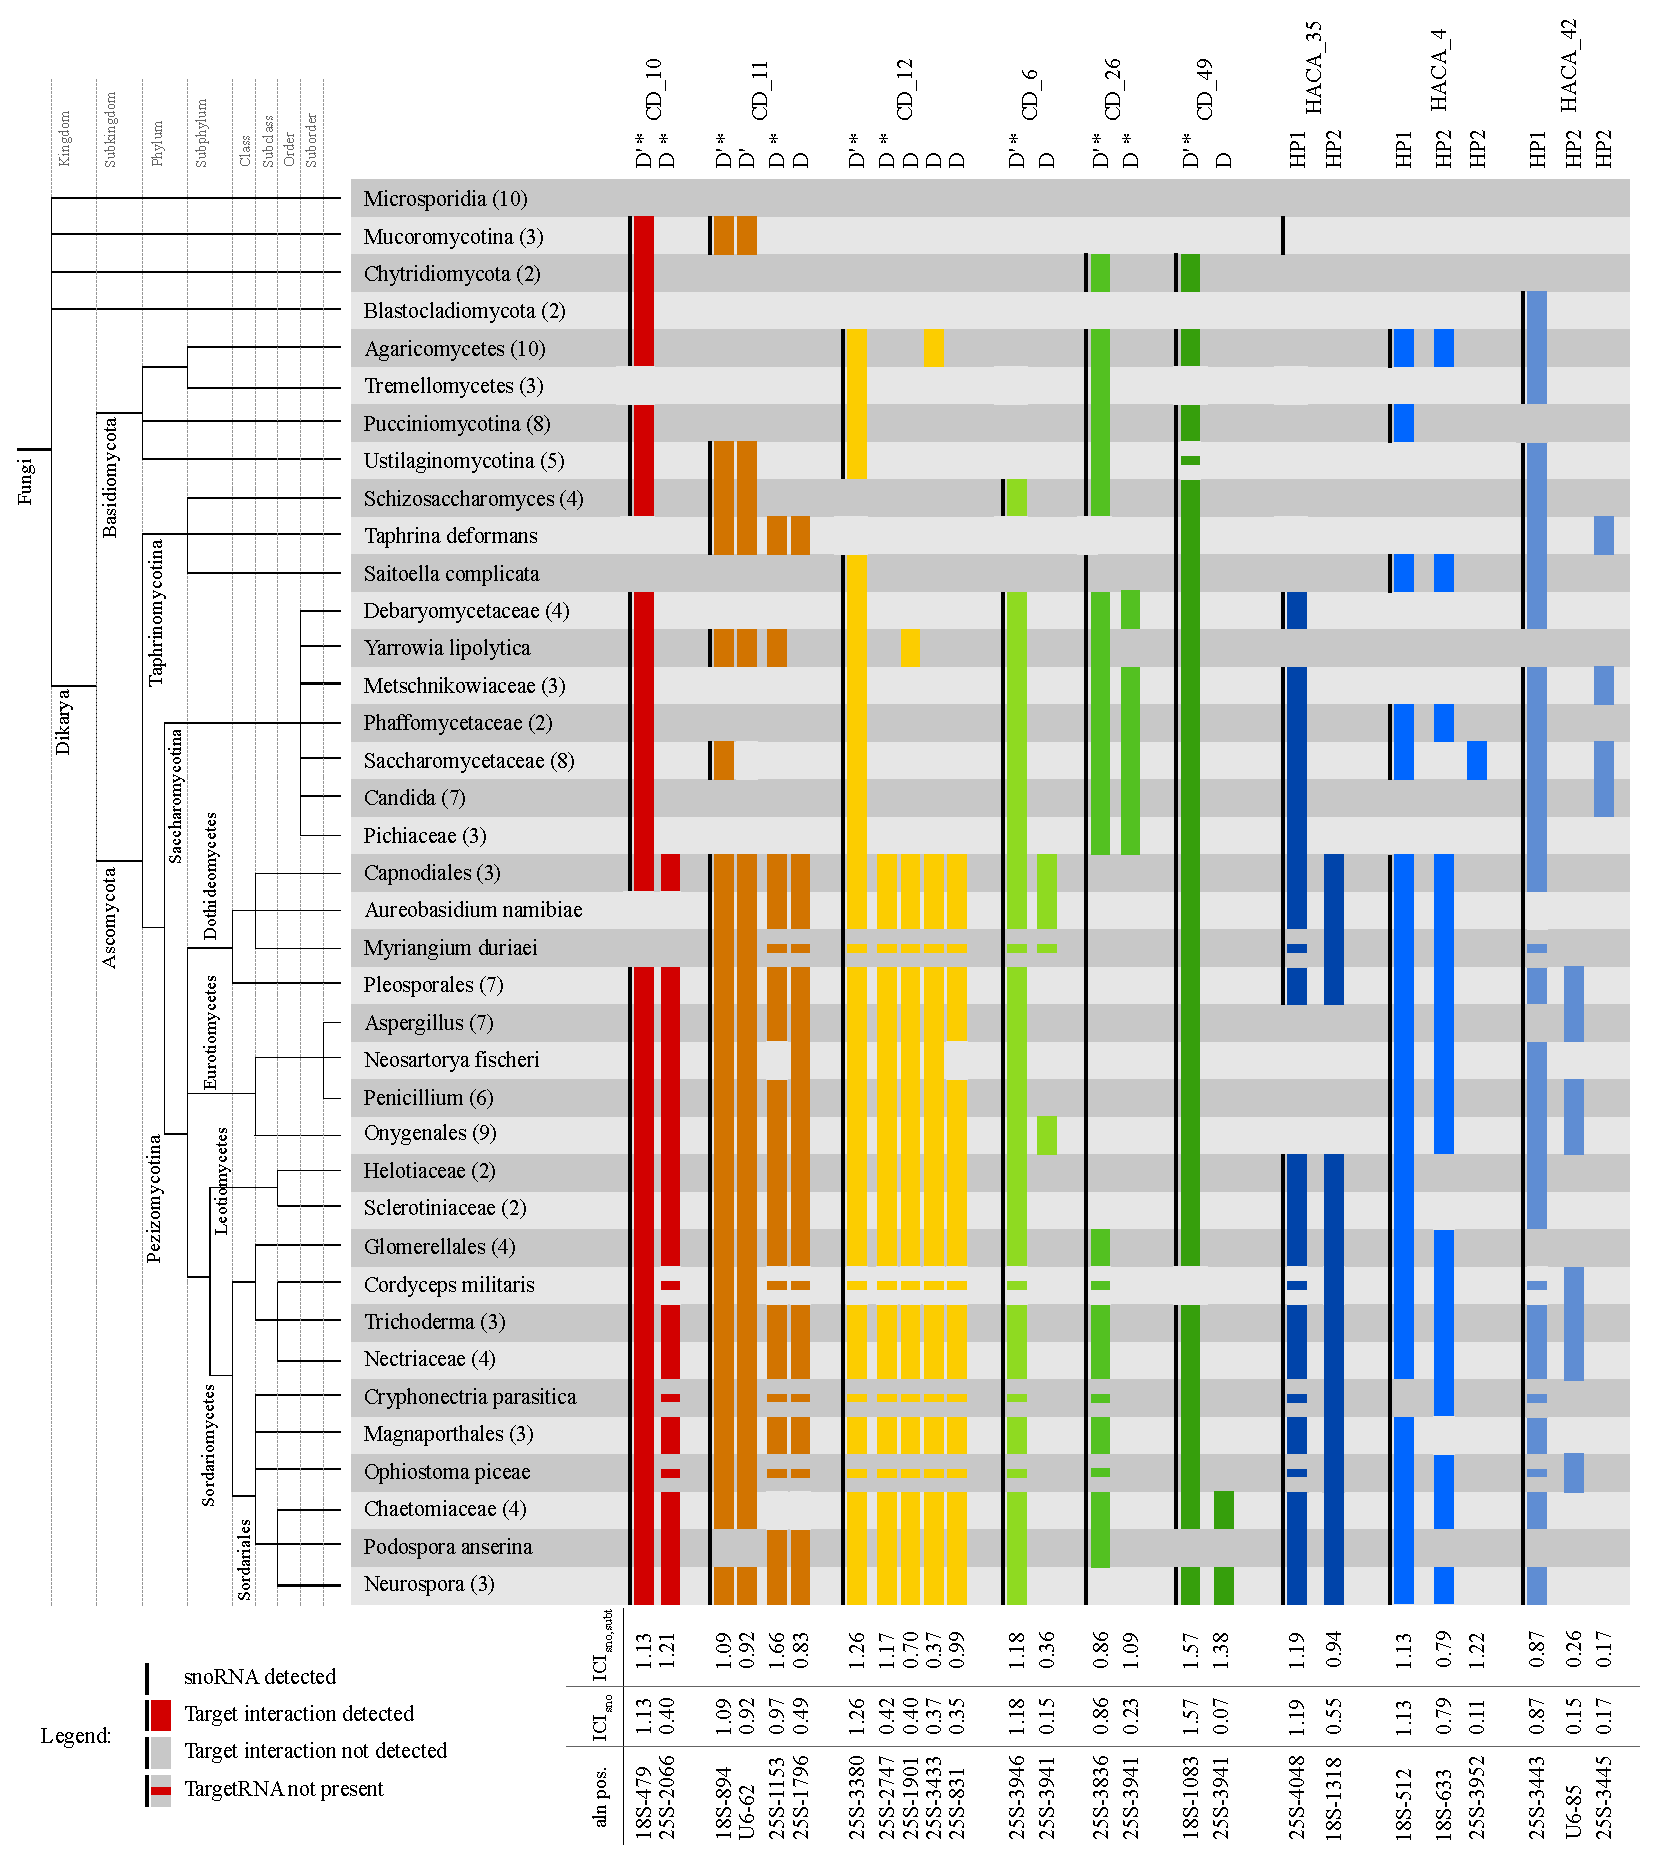
\includegraphics[width=\textwidth]{pics/conservation_lineage_specific_targets.eps}
  \caption{The conservation of predicted target interactions is shown for
    interesting single guide \cd\ families that exhibit an additional
    functional target at their 'non-functional' D box. Each family is
    depicted in a different color. The black bar in front of each
    family shows the presence of the family in a certain lineage or
    organism. The color bar shows that at least one target interaction
    was predicted in that lineage. The respective family name and target
    site can be seen on top while the alignment position and the
    corresponding ICI score are shown at the bottom. Experimentally
    confirmed interactions are denoted with '*'.}
  \label{fig:additional_targets}
\end{figure*}

Interesting \cd\ families with a previously annotated functional D'
targets and lineage specific D targets can be seen in Figure
\ref{fig:additional_targets}. Detailed information about all \sno\
families with an additional, lineage specific target are found in the supplement.

Family CD\_10, for example, with its experimentally verified target 18S-479
(\sce\ snR87; 18S-436; D' target), is detected in all analyzed fungal
lineages except for Microsporidia. Besides the functional D' region,
all Pezizomycotina species, whose large subunit rRNA is available, are
also predicted to guide an additional target upstream of their D
box. The target 25S-2066 (\ncr\ 25S-1042) has an ICI$_{sno}$ score of
1.21 amongst members in the Pezizomycotina subtree. The mean mfe is -13.19 kcal/mol.
CD\_11 was shown to guide the methylation at position 18S-894 (\sce\ snR53;
18S-796; D' target) in the budding yeast. The \snostrip-analysis
confirmed the \sno\ and this specific target interaction in a wide
range of fungi. An additional D' target, U6-62 (\sce\ U6-45), was
originally published in \ncr\ \cite{Liu:2009} based on single sequence
prediction. This interaction is also convincingly 
confirmed by \snostrip\ in all \sno s that were previously found to guide the
18S-894 target, except for Saccharomycetaceae, see Figure
\ref{fig:additional_targets}. Position 45 in U6 snRNA was not found to
be modified in the budding yeast
\cite{Machnicka:2013, Massenet:1998}. Due to missing analyses, no such
statement can be made in most other
fungal species. Since the ICI score for the U6 target is only marginal
smaller than for the 18S target, 0.89 to 0.94, respectively, and the
mean mfe value is found to be -13.78 kcal/mol (18S-894: -17.34), it is
thoroughly possible that this \sno\ is capable of modifying both
targets. However, two additional targets can be found for
the ASE upstream of box D: 25S-1153 and 25S-1796 (\ncr\ 25S-359 and
25S-790). Both candidates are predicted throughout all Pezizomycotina
species and, surprisingly, \Tde, a relative to the fission yeast. The
first interaction is additionally found in \Yli, a close
relative to the budding yeast. Because of its extraordinary low mean
minimum free energy of -21.12 kcal/mol, this target is assigned a high
ICI value of 1.66. The second putative interaction has an ICI score of
0.83 and a mean mfe of -11.50.

A highly interesting modification site is 25S-3941 (\sce\ 25S-2724)
whose actual methylation and the guidance by snR67 (\sce) was experimentally shown
\cite{Lowe:1999}. The conserved interaction of this position is
traceable in at least three different families, each in another fungal
lineage. Family CD\_26, which contains the budding yeast
sequence, shares a conserved D' target 25S-3836 (\sce\ 25S-2619)
that is predictable in all Dikarya except for Dothideomycetes,
Eurotiomycetes, and Leotiomycetes (ICI: 0.86, mean mfe: -23.03
kcal/mol). The D target 25S-3941, on the other hand,
is solely found in Saccharomycotina (ICI: 1.09, mean mfe: -15.34). Family CD\_6 is found to share this target as a conserved D box
interaction in Onygenales and in a part of Dothideomycetes (ICI: 0.36, mean mfe:
-15.46). In a third family, CD\_49, the
modification at 25S-3941 is predicted in Sordariales (ICI: 1.38, mean
mfe: -14.14).
%These scattered interaction might have two different
%explanations; the interaction was either a subject of different target
%switches or it was completely lost at some point in fungal
%evolution. The latter scenario might have caused severe effects in
%development or growth of certain species such that the interaction
%might be reinvented in different lineages. However, either way
%indicates an importance for this specific methylation. 

In similarity to the box C/D \sno\ class, several \haca s comprise a
functional and highly conserved target guiding region in one hairpin
and show lineage-specificity in the other, see Figure \ref{fig:additional_targets}. 
Again, a detailed summary can be found in the
supplement. Some of these functions might already been annotated, 
especially in \sno\ sequences of the budding yeast, see families
HACA\_4 and HACA\_42 which are in fact officially denoted as double guides
in \sce. Both families show an interesting pattern in their second
hairpins.  HP1 is highly conserved in both cases and the corresponding
target binding capability is at least present in Dikarya. In their second hairpin,
however, they developed two different guiding functions that are
predictable in separate lineages. HACA\_4, for example, is known to
guide the pseudouridylation at 25S-3952 in Saccharomycetaceae while
outside of this clade the \sno\ is mostly predicted to guide modification
at 18S-633. In HACA\_42, on the other hand, the separation of both
target guiding functions becomes even more conspicuous. The budding yeast
annotated modification site is predicted in Saccharomycotina and \Tde\
(25S-3445), whereas the position U6-85 is predicted in a wide range of
Pezizomycotina.

Family HACA\_21 is
predicted to guide the modification at position 57 (\ncr\ 54, \sce\ 54) in the
5.8S rRNA with its first hairpin in a large amount of Pezizomycotina
species (ICI$_{sub}$ = 0.73). This particular modification is not present in budding yeast
5.8S molecules which undoubtedly explains the missing predictions in
this subtree. On the contrary, the corresponding human position is found to
be pseudouridylated raising the possibility for this predicted
interaction to be an authentic and biological correct modification.
Based on the ICI$_{sub}$ score, a potential, alternative target at
position 25S-2813 is convincingly predicted with 1.07 in 19 out of
27 Saccharomycetales organisms. Since experimental evidence for this
precise position is missing, the prediction remains hypothetical.

\paragraph{\textbf{Target switches}}
Occasionally during evolution, novel guiding interactions are acquired
or present ones are lost in different species or lineages. It is,
however, much more uncommon that some target interactions are
translocated from one snoRNA to another. Therein, the position of the ASE
within the snoRNA sequence, upstream of box D/D’ or in HP1/HP2, is mostly
preserved but it happens seldomly that this position is also
shifted. Two highly complex rearrangements have been autmatically
detected by \snostrip. Each of these two '\sno\ clans' comprise two,
three or even more \sno\ sequences in each organism with distinct
target interactions. Due to target switches during fungal evolution,
these previously independent \sno\ sequences became connected. Table
\ref{tab:sno_clans} summarizes the target interactions that are convincingly predicted in the \sno\ clans CD\_5 and CD\_19.
\begin{table}
  \caption{Interaction properties of four LSU modifications of CD\_5
    are shown. Properties for three SSU and two LSU methylations are
    given for clan CD\_19.}
  \label{tab:sno_clans}
\begin{center}
  \begin{scriptsize}
  \begin{tabular}{c|c|c|c|c}
    &&&&detected\\
    & \raisebox{1.5ex}[1.5ex]{modification}& \raisebox{1.5ex}[1.5ex]{ICI$_{sno}$}& \raisebox{1.5ex}[1.5ex]{$\varnothing$ mfe}&interactions\\
  \hline
  &25S-1806&0.79&-16.46&23.08\%\\
  &25S-1866&0.90&-19.49&24.61\%\\
  \raisebox{1ex}[3ex]{\rotatebox{90}{CD\_5}}&25S-1898&1.20&-25.80&25.38\%\\
  &25S-3615&1.00&-18.48&25.77\%\\
  \hline
  &18S-462&1.52&-20.62&34.49\%\\
  &18S-602&1.11&-15.30&34.18\%\\
  \raisebox{-2ex}[3ex]{\rotatebox{90}{CD\_19}}&18S-1580&1.75&-20.76&34.49\%\\
  &25S-2574&0.48&-22.85&9.49\%\\
  &25S-4143&0.28&-15.49&7.59\%\\
  \end{tabular}
  \end{scriptsize}
  \end{center}
\end{table}

In the following, we will focus on the description of the \sno\ clan
CD\_5. The potential evolutionary history of CD\_19 is exlained and
illustrated in the supplement.  

\begin{figure*}
  \centering
  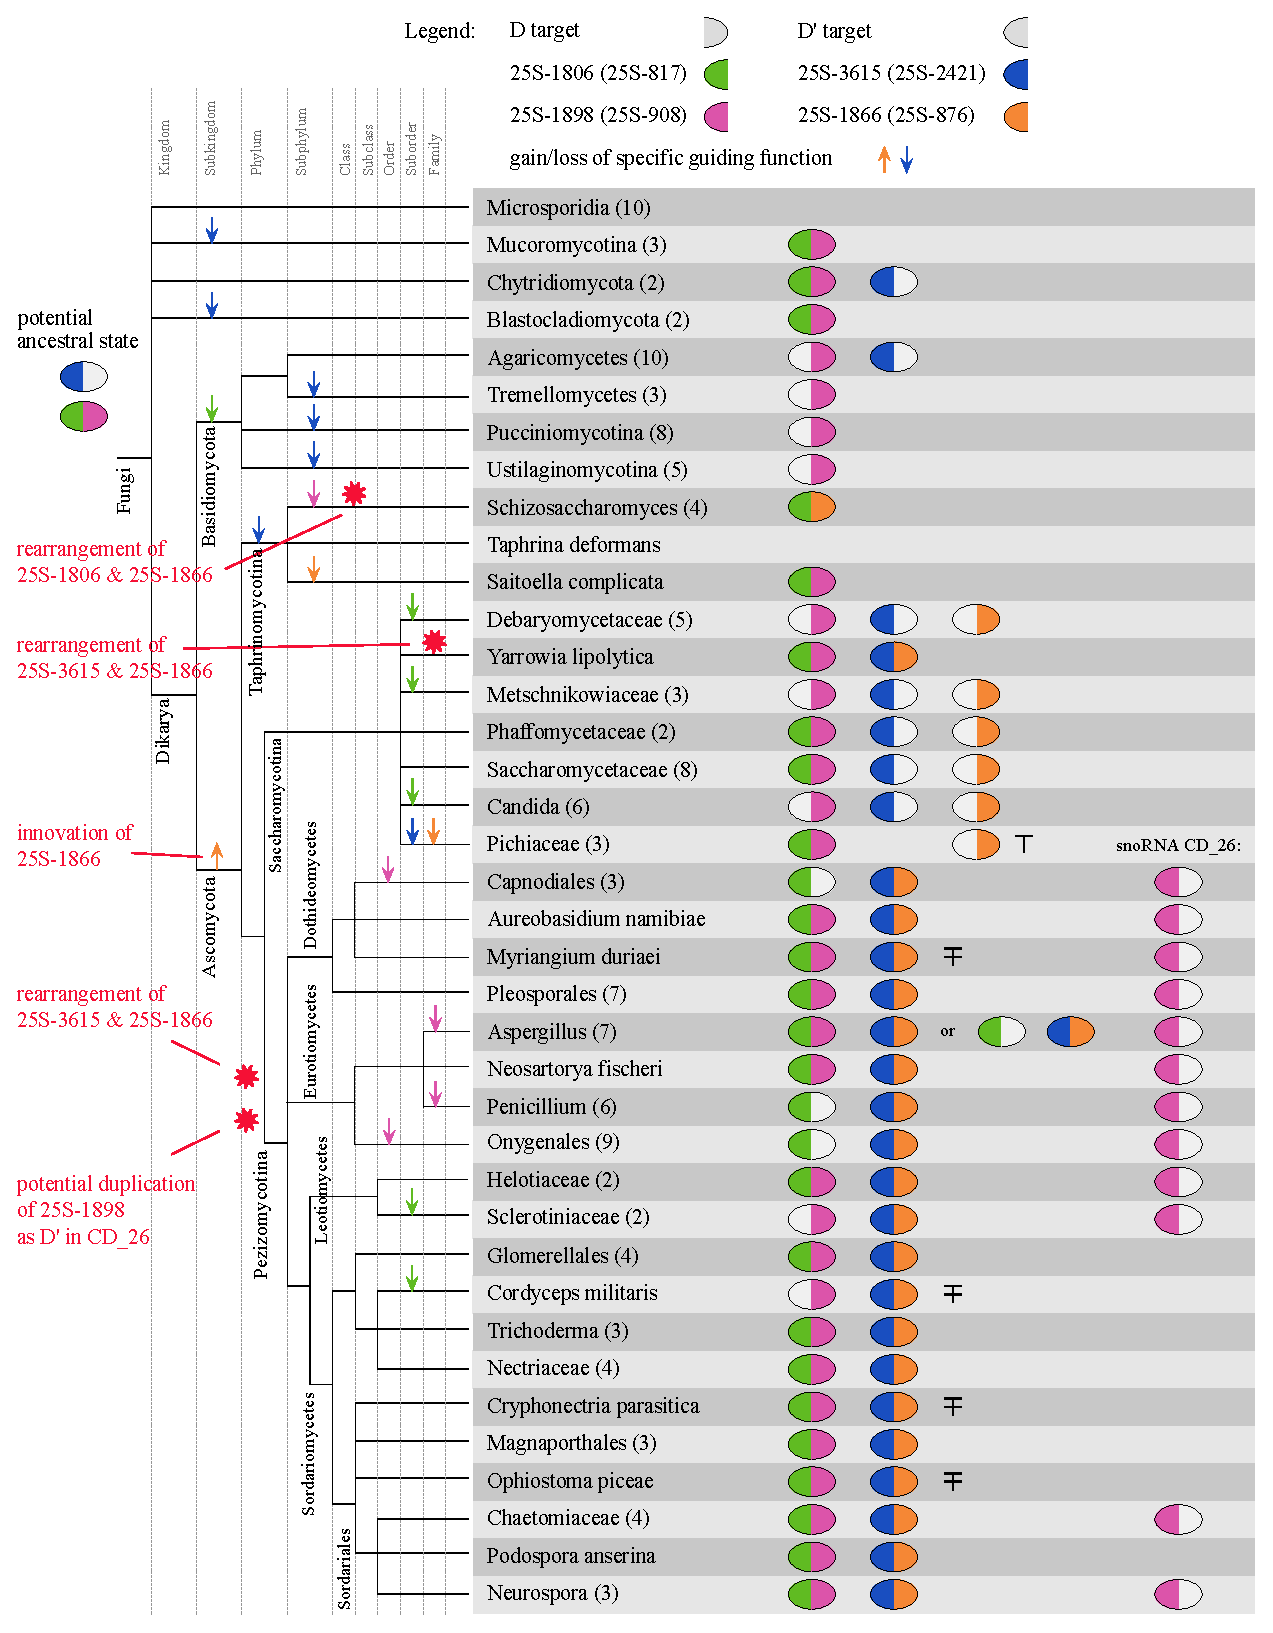
\includegraphics[width=0.9\textwidth]{pics/target_switches_CD_5.eps}
  \caption[Potential evolutionary history of \sno\ clan
  CD\_5.]{Potential evolutionary history of \sno\ clan CD\_5 involving
  four modification sites on the LSU rRNA. Gain/loss events
  are displayed with arrows, while potential rearrangements are shown
  with red stars. $\top$ 25S-1866 is solely found in Pichia. $\mp$ Putative since LSU sequences are missing; \sno s show convincing
ASE conservation.}
  \label{fig:CD_5}
\end{figure*}

\textbf{The \sno\ clan CD\_5} comprises three distinct budding yeast \sno\
sequences (snR60, snR72, and snR78) which at first sight do not share
a common evolutionary background. snR60 was verified to guide
methylations at 25S-1898 (single sequence 25S-908, D target) and
25S-1806 (25S-817, D' target), snR72 guides the methylation at
25S-1866 (25S-876, D target), and snR78 was shown to direct the
modification at position 25S-3615 (25S-2421, D' target). The
methylations at position 25S-1806, 25S-1898, and 25S-3915 map to known
and verified modifications in human large subunit ribosomal RNAs and
hence, are supposed to be ancient, which in consequence suggest the real existence
of both the methylations and the guiding snoRNAs at the root of fungi.
However, through individual target switches in the cause of fungal
evolution, the history of these sequences became connected. A
taxonomic tree displaying a potential evolutionary history involving
\sno s that are predicted to guide the above mentioned modifications is shown in
Figure \ref{fig:CD_5}. Therein, the putative ancient state is
described to be constituted of two individual \sno\
sequences guiding the three ancient methylations. 
Parsimonious deletion and innovation events of target interactions are marked
accordingly. The emergence of the fourth modification, 25S-1866, is
predicted at the root of Ascomycota, since all diverging
lineages are either predicted or verified to target this specific
site. The loss of any of the four guiding functions occurred rather
frequently in several lineages, e.g., Basidiomycota are supposed to
have lost the guiding potential for 25S-1806 while different
Basidiomycota lineages are further predicted to have lost the ability
to guide methylation at 25S-3615.

\begin{figure*}
  \centering
  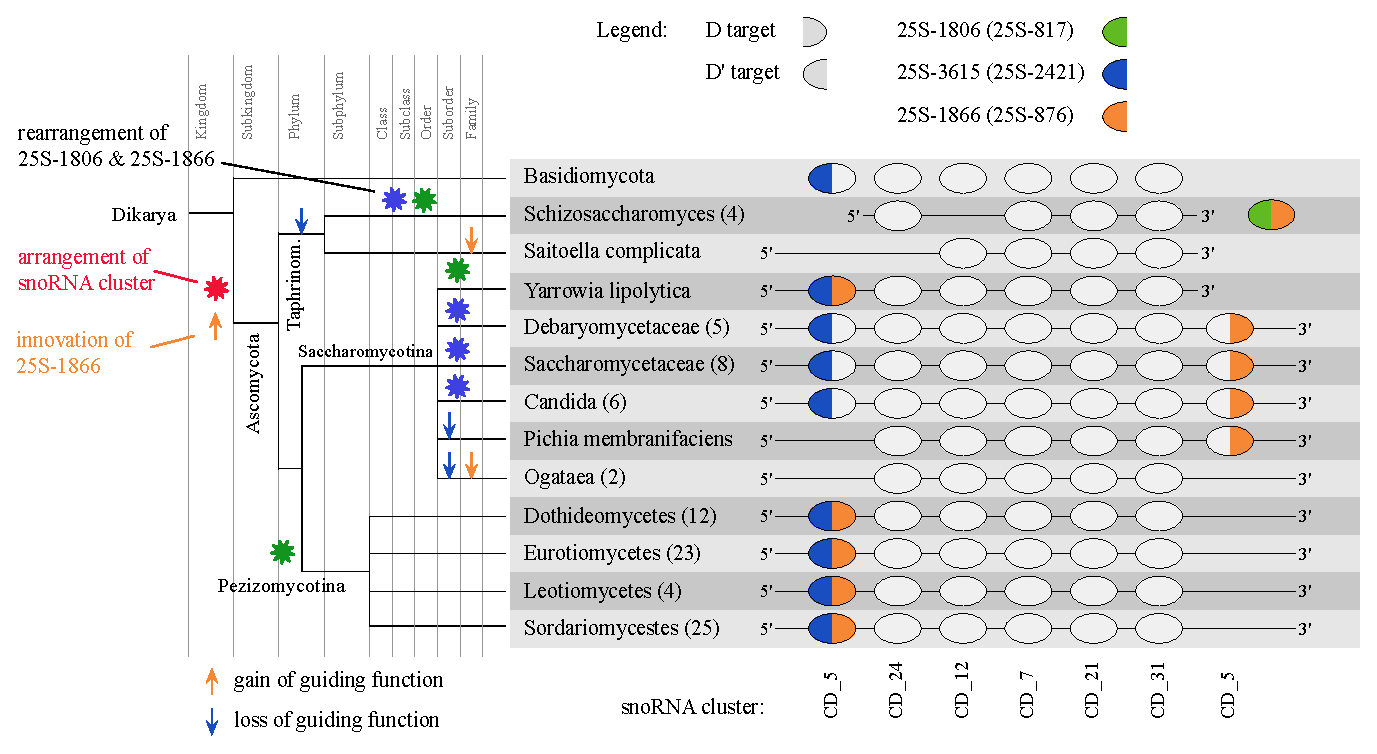
\includegraphics[width=\textwidth]{pics/target_switches_CD_5_cluster.eps}
  \caption[Evolution of a \sno\ cluster harboring CD\_5
  sequences.]{Sequences of the CD\_5 \sno\ family are incorporate into
  a polycistronic transcript that harbors up to seven \sno\
  genes. This cluster with its highly conserved structure and size occurred at the root of Ascomycota, but most of
  its genes arose at least at the root of Dikarya. There are different
  potential histories regarding the evolution of the cluster depending on how
  the newly innovated target guiding function at position 25S-1866
  (orange) was initially introduced in this polycistronic
  transcript. A) Evolutionary history under the assumption that
  25S-1866 is incorporated as a second guiding function into the \sno\
  guiding 25S-3615. B) History under the hypothesis that a novel
  single guide \sno\ is introduced at the 3' end of the \sno\
  cluster. The most parsimonious rearrangement events that led to the
  observed cluster organization are depicted in
  blue and green stars, according to hypothesis A and B, respectively.}
\label{fig:CD_5_cluster_history}
\end{figure*}

Besides such ordinary processes of gain and loss events, it happened
several times during fungal evolution that target interactions
of the mentioned four modifications switched between different \sno s.
It is a noteworthy fact that the actual target site within the \sno\
(D' or D target) are mostly preserved. Within the Taphrinomycotina
lineage, including the fission yeast, target guiding functions at
25S-1806 (D' target) and 25S-1866 (D target) are incorporated into one \sno\ sequence after
the original guidance of 25S-1898 (D target) went missing. 

At the root of Ascomycota, a polycistronic \sno\ transcript is
arranged including the \sno\ sequences of CD\_24, CD\_12,
CD\_7 CD\_21, and CD\_31 in 5'-3' direction, see Figure
\ref{fig:CD_5_cluster_history}.  All these \sno\ families
are already present at the root of Dikarya, distributed over large
distances or different chromosomes. After the formation of this
cluster, the precise order and the
length of approx. 1.5kb is highly conserved throughout all
Ascomycota. 

It might have happened that a \sno\ of clan CD\_5 guiding
methylation at 25S-3615 is already present at the 5' end of this
cluster when it emerged. However, there are several possibilities how
the \sno\ cluster evolved after the innovation of guiding function for 25S-1866. 
One hypothesis (Blue stars in Figure \ref{fig:CD_5_cluster_history}) is the initial incorporation of 25S-1866 into the \sno\
that already guides 25S-3615, creating a double guide \sno at the 5'
end of the polycistronic transcript. In Taphrinomycotina, the loss of
guiding function for 25S-3915 and 25S-1898  might have caused the
rearrangement of the 25S-1806 and 25S-1866 and the exclusion from the
\sno\ cluster. At the root of Saccharomycotina, the double guide \sno\
might have split up leaving a single guide at the 5' end (25S-3615)
and a novel single guide at the 3' end of the cluster
(25S-1866). The original formation is solely conserved in
\Yli. In another hypothesis, evolution might have taken the other
way round (green stars in Figure
\ref{fig:CD_5_cluster_history}). Assuming the innovation of 25S-1866
led to a novel single guide \sno\ that is located at the 3' end of the
\sno\ cluster, as seen in Saccharomycetaceae, \yli\ would be the only
organism in Saccharomycotina where a  rearrangement is detected. In
result, the previously single guide sequences are reorganized into a
double guide sequence  with guiding ability for
25S-3615 as D' target and 25S-1866 as D target. This novel double guide is now located at the 5' end of the
cluster. 
Coincidentally, the same reorganization happened at the root
of Pezizomycotina, where the first \sno\ of the cluster is found to
guide modifications at position 25S-3615 (D') and 25S-1866
(D). Proteins that are located up- and downstream of the previously
described \sno\ cluster are not found to be conserved throughout major
fungal lineages.


A further interesting observation is the potential duplication of
target interaction for 25S-1898 at the root of Pezizomycotina. This
ability is inserted into family CD\_26 as a D' target in the lineages
Dothideomycetes, Eurotiomycetes, and Leotiomycetes
(ICI$_{Pezizomycotina}$: 1.13, mean
mfe: -18.79). Neurospora species
are also predicted to guide this methylation with its CD\_26 \sno. In reverse the
original D' target of CD\_26, 25S-3836, was abolished in these
organisms and is not found to be restored in any other \sno\ family.
Please also confer Figure \ref{fig:additional_targets} for more
detailed information of family CD\_26. The invention of redundant
guides would explain the findings that in some of these species the original target
site of 25S-1898 vanished in CD\_5 \sno s, e.g., in Capnodiales, some Aspergillus
organisms, or Onygenales. Families CD\_5 and CD\_26 are not merged due
to a switch of the ASE (from D in CD\_5 to D' in CD\_26). 





\paragraph{\textbf{Multiple Target Interactions}}
It might happen, that \sno\ families are not only convincingly
predicted to guide one specific target modification but two or even
more with the same ASE.
\begin{table}
  \caption{Summary on
    multiple target predictions of families CD\_43 and CD\_61 that are guided with the same ASE.}
  \label{tab:redundant_predictions}
  \begin{center}
    \begin{footnotesize}
      \begin{tabular}{c|c|c|c|c}
        &pos&ICI$_{sno}$&$\varnothing$
          mfe&\# ia\\
        \hline
        &18S-1400&0.95&-12.96&67/90\\
        \raisebox{1.5ex}[-1.5ex]{CD\_43}&18S-614&1.61&-21.96&71/90\\
        \hline
        &18S-1843&1.48&-17.82&86/102\\
        &5.8S-155&1.16&-12.99&92/102\\
        CD\_61&18S-348&1.04&-12.99&83/102\\
        &18S-1827&1.02&-12.49&85/102\\
        &5.8S-120&1.00&-11.36&91/102\\
      \end{tabular}
    \end{footnotesize}
  \end{center}
\end{table}
An outstanding example is given by \cd\ family
CD\_43 (\sce\ snR40) which is predicted and experimentally validated to guide
methylation at position 18S-1400 (18S-1271) with its D' target binding
region. This interaction is predicted in 67 out of 90 \sno s and provides
an ICI score of 0.95 with a mean interaction energy of -12.96
kcal/mol. However, an even better target is predicted at position
18S-614 (18S-562) with an ICI score of 1.61 and a mean mfe of
-21.69. This interaction is found in 71 organisms. All 67 \sno s
predicted to guide the first target are also predicted to guide the
latter one, in a vast majority of cases even with a better binding
energy. But since the genuine modification is neither reported in
\sce, \ncr, or human, this prediction, albeit its overly convincing
nature, remains hypothetical. 

An even more vital example is provided by family CD\_61 (D' ASE).
Not less than five potential targets are predicted with an ICI score
above 1.0, a mean mfe below -11.30 and more than 80 single sequence
predictions. Details are shown in Table
\ref{tab:redundant_predictions}. This time, the most persuasive
prediction is experimentally confirmed, whereas the other predicted
positions were not shown to be modified yet. 

% --------------------------------------------------------------------------- %

\section{Discussion}

We provide here a comprehensive inventory of snoRNAs in fungi together with
an in-depth analysis of the evolution of snoRNA families and their target
specificities. The investigation of 147 different taxa provides a detailed
history of gain, loss, and duplication events for 68 families of box C/D
snoRNAs and 50 families of box H/ACA snoRNAs involving more than 7,700
individual snoRNA sequences. \PFS{For 18 snoRNA families previously
unrecognized homology with other families has been uncovered. These data
constitute a substantial extension and refinement of the accumulated
knowledge on \sno{}s. Data and refined models will become available in the
\rfam\ database and collectively form an important step towards a global
understanding of the evolution of the snoRNAome. Since our approach is
based on homology search, it is fundamentally limited by the seed sequences
that have been observed and classified as \sno{}s in at least one
organism. It is very unlikely, therefore, that this study presents a
complete picture despite 
%doubling the number of \sno\ families and
increasing the number \sno\ sequences by more than a factor of
four. Additionally, for 26 of 39 orphan \sno s (including sequences
with single-sequence target predictions only) could be mapped to
experimentally 
verified targets or a least a quite convincing prediction based on the
Interaction Conservation Index (ICI)
could be assigned.}


The processing of this amount data is well beyond the realm of manual
curation and has been possible only with the help of \snostrip, a pipeline
specifically developed to investigate the evolution of snoRNA families
across a broad phylogenetic range \cite{Bartschat:2014}.  The in-depth
analysis of potential target interactions adds a new layer of
information. We have demonstrated here that the coevolution of \sno s and
their targets can be tracked with high resolution based on the functional
characteristics of the \sno s as determined by \snostrip\ together with a
quantitative assessment of predicted RNA-RNA interaction based on the the
Interaction Conservation Index (ICI) \cite{Kehr:2014}.

Similar to Metazoa, fungal \haca s show a higher loss-ratio compared
to \cd s. This might have both a technical and a biological
explanation that manifests itself on two different levels. Since \haca
s do not share long ASEs but rather short bipartite pseudouridylation
pockets, it becomes considerably harder to detect homologous \sno s
over large evolutionary timescales. This effect may limit the
scope of the homology search procedure. The short interacting regions
also make these molecules more vulnerable to mutations that disrupt
the snoRNA-targetRNA interaction. At the same time, the presence of
the second, independent ASE in the other hairpin may be a sufficient
cause to retain mutated genes.

In general, fungal \sno s have well preserved target interactions and
most families are found to contain exactly one highly conserved
anti-sense element. The remaining target region is in turn free to
evolve or to adapt to new lineage-specific or even species-specific
targets. Here we introduced a variation on the ICI scoring adapted to
subclades, allowing a much more detailed quantitative assessment of
target turnover. Many of the predictions made here of course await
experimental validation, given that experimental evidence for
RNA-target interactions as well as direct measurements of chemical
modifications in the primary target molecules (rRNAs and snRNAs) are
still restricted to a few model organisms.

The computational analysis reported here strongly suggests that
snoRNAs not only address a highly conserved ASE but also frequently
have additional, secondary targets. The possibility that a single
\sno\ target site exerts two distinct guiding functions has been
reported from budding yeast \haca s. The budding yeast \sno\ family
snR3 (HACA\_3), for example, is verified to target two modification
sites in its second hairpin \cite{Schattner:2004}.  Both interactions
can be tracked across the Dikarya.  Nevertheless, there is still very
little experimental data on the generality of this effect and most of
the predicted 'double' target sites will still require experimental
verification. Convincing examples of remarkably conserved multiple
interactions are found in \cd\ families snR40 (CD\_43) and snR70
(CD\_61), which exhibit two and five high-scoring target-interactions
at a single ASE, respectively.  These findings suggest the possibility
that \sno s are, at least under certain circumstances, able to guide
different modifications with the same ASE. This might be dependent on
developmental phases, or more complex mechanisms involving
conformational changes of the target.

In some cases of \haca s, these additional targets exhibit better ICI
scores than the annotated modification sites. Since the ICI combines
evidence from thermodynamic stability and evolutionary conservation, these
predictions cannot be easily dismissed as false positives. The specialized
ribosome hypothesis proposes distinct ribosomal conformations in different
developmental stages and stress levels that might also entail different
chemical modification patterns of the rRNAs; it is entirely plausible in
this scenario that some modifications and thus snoRNA interaction sites
have remained undetected \citep{Xue:2012}. The existence of
stress-induced conditional pseudouridylations indeed has been reported for
the for the U2 snRNA of budding yeast \cite{Wu:2011}. The snR81 RNA, which
is also responsible for guidance of a constitutive U2 pseudouridylation,
guides one of the novel modifications through imperfect and redundant base
pairing. The authors speculate that conditionally induced modifications in
RNA may well be a rather frequent phenomenon.

On the other hand, we also found convincing evidence that some
modifications are guided by two, three, or even more \sno\
families. First, this includes redundant guides, meaning that two
snoRNA families of the same species are responsible for the same
modification. Second, we observed several target sites that are
addressed by different snoRNA families in different taxonomic
groups. A good example for the latter situation is the predicted
pseudouridine at position 5.8S-18. Although there is not direct
experimental evidence that this particular position is modified
\emph{in vivo}, the site is predicted as a target for several distinct
snoRNA families by \snoop\ (see supplement section S21).

The fact that specific modification sites are predicted to be guided
by more than just one \sno\ family in the same organism has several
possible reasons. SnoRNA expression recently was reported to be
strongly regulated in development and between tissues or cell lines
\cite{Kapushesky:2012, Jorjani:2016}. It may thus be necessary for the
organism to compensate for snoRNAs that are lowly expressed under
certain circumstances to maintain the functional modification levels
of the target RNA. This may be achieved by means of paralog or through
the redundant target binding capability of another \sno\ family.

In summary we observe that the landscape of snoRNAs keeps changing
over the the evolutionary time-scale of the kingdom Fungi. We observe
both the extinction of entire \sno\ families and the innovation of new
ones. The function of snoRNA families itself also changes at these
evolutionary scales, showing loss, gain, and turn-over of guiding
functions that lead to target switches. The number of known snoRNA
families in Fungi is lower than in animals, correlating well with the
observation that animals have more (reported) modification sites in
their rRNAs and snRNAs than ``lower'' Eukaryotes (see
\texttt{Modomics} and the \texttt{RNA Modification Database}
\cite{Machnicka:2013, Cantara:2011}) or even Bacteria (which have
target-specific enzymes for each individual modification instead of
the generic enzyme machinery with snoRNAs as evolutionary flexible
``address labels'').

On the other hand, there are many similarities between the fungal and
the metazoan snoRNAome.  A common feature is the detectable burst in
the \sno\ diversity at each major branching point in the taxonomic
tree of both kingdoms.  In case of \cd s, the distribution of orphan,
single guided, and double guided \snos\ is quite similar compared
between fungi and animals, as reported by the human \sno\ atlas
\citep{Jorjani:2016}: Over 70\% of the human box C/D carrying \sno s
are found to be single guided (75\% in Fungi).  In both human and
fungi the remainder is about equally split between double guided and
orphan snoRNAs. The situation is somewhat different for \haca s: in
human double guided \sno s comprise the largest group (47\%), while in
Fungi, only 22\% of the \haca\ families target two distinct
pseudouridylation sites with both hairpins.



% --------------------------------------------------------------------------- %

\section*{Acknowledgments}

This work was funded in part by the European Union FP-7 project QUANTOMICS
(no.\ 222664), the MMML-seq project of the International Cancer Genome
Consortium (ICGC) funded by German Federal Ministry of Education and
Research, the CRC 1052 ``Obesity'', and by the Deutsche
Forschungsgemeinschaft (Project DFG STA 850/15-1). LIFE -- Leipzig Research
Center for Civilization Diseases is funded by the State of Saxony and the
European Union.

\bibliographystyle{m}
\bibliography{Fungi_snoRNAome}

\end{document}


